% Tarea 2: Numeros pseudoaleatorios y metodos de Monte Carlo
% Compilar desde doc/ con:  tectonic -X compile tarea2.tex
% Antes hay que correr los scripts de src/ para generar figuras y tablas.
\documentclass[11pt,letterpaper]{article}

\usepackage[utf8]{inputenc}
\usepackage[T1]{fontenc}
\usepackage[spanish,es-tabla]{babel}
\usepackage{amsmath,amssymb,amsthm}
\usepackage{graphicx}
\usepackage{booktabs}
\usepackage[margin=2.4cm]{geometry}
\usepackage{xcolor}
\usepackage[most]{tcolorbox}
\usepackage{enumitem}
\usepackage{caption}
\usepackage{parskip}
\setlength{\parskip}{0.75em plus 0.2em minus 0.1em}
\usepackage[hidelinks]{hyperref}

\graphicspath{{../figs/}{figs/}{./}}

% Generado por src/part1_generators.py.
% No editar a mano: se sobrescribe en cada ejecucion.
\newcommand{\NMuestra}{100{,}000}
\newcommand{\NTernas}{3{,}000}
\newcommand{\Semilla}{141903}
\newcommand{\SemillaBBS}{14773}
\newcommand{\PlanosRandu}{15}
\newcommand{\ResiduoRandu}{$0$}
\newcommand{\statChiLCG}{6.17}
\newcommand{\pChiLCG}{0.7223}
\newcommand{\statKSLCG}{0.00312}
\newcommand{\pKSLCG}{0.2830}
\newcommand{\statLagLCG}{+0.00119}
\newcommand{\pLagLCG}{0.7075}
\newcommand{\statRachasLCG}{49{,}849}
\newcommand{\pRachasLCG}{0.3364}
\newcommand{\velLCG}{3{,}045{,}229}
\newcommand{\statChiCM}{748369.88}
\newcommand{\pChiCM}{0.0000}
\newcommand{\statKSCM}{0.91138}
\newcommand{\pKSCM}{0.0000}
\newcommand{\statLagCM}{+0.73241}
\newcommand{\pLagCM}{0.0000}
\newcommand{\statRachasCM}{0}
\newcommand{\pRachasCM}{0.0000}
\newcommand{\velCM}{1{,}655{,}135}
\newcommand{\statChiMT}{6.51}
\newcommand{\pChiMT}{0.6879}
\newcommand{\statKSMT}{0.00303}
\newcommand{\pKSMT}{0.3175}
\newcommand{\statLagMT}{+0.00245}
\newcommand{\pLagMT}{0.4393}
\newcommand{\statRachasMT}{49{,}904}
\newcommand{\pRachasMT}{0.5396}
\newcommand{\velMT}{982{,}384}
\newcommand{\statChiBBS}{3.27}
\newcommand{\pChiBBS}{0.9527}
\newcommand{\statKSBBS}{0.00132}
\newcommand{\pKSBBS}{0.9948}
\newcommand{\statLagBBS}{+0.00048}
\newcommand{\pLagBBS}{0.8786}
\newcommand{\statRachasBBS}{49{,}993}
\newcommand{\pRachasBBS}{0.9596}
\newcommand{\velBBS}{369{,}097}
\newcommand{\statChiRANDU}{8.80}
\newcommand{\pChiRANDU}{0.4561}
\newcommand{\statKSRANDU}{0.00220}
\newcommand{\pKSRANDU}{0.7185}
\newcommand{\statLagRANDU}{-0.00024}
\newcommand{\pLagRANDU}{0.9390}
\newcommand{\statRachasRANDU}{50{,}136}
\newcommand{\pRachasRANDU}{0.3932}
\newcommand{\velRANDU}{3{,}207{,}784}
\newcommand{\CMColapso}{8{,}864}
\newcommand{\CMFracCeros}{91.1\%}
\newcommand{\CMLargoMin}{22}
\newcommand{\CMLargoMax}{16{,}072}
\newcommand{\CMLargoMedio}{4{,}625}
\newcommand{\CMCiclo}{1}
\newcommand{\CMUtilN}{8{,}864}
\newcommand{\CMUtilChi}{5.31}
\newcommand{\CMUtilChiP}{0.257}
\newcommand{\CMUtilKS}{0.0092}
\newcommand{\CMUtilKSP}{0.443}
\newcommand{\MTIdentico}{si}

% Generado por los scripts de src/.
% No editar a mano: se sobrescribe en cada ejecucion.
\newcommand{\NFinal}{1{,}000{,}000}
\newcommand{\Repeticiones}{10}
\newcommand{\ExactoSeno}{0.636620}
\newcommand{\ExactoNormal}{0.477250}
\newcommand{\EstSeno}{0.637334}
\newcommand{\ICSeno}{[0.636731,\ 0.637937]}
\newcommand{\ErrorSeno}{$7.1\times 10^{-4}$}
\newcommand{\EstNormal}{0.477344}
\newcommand{\ICNormal}{[0.476893,\ 0.477795]}
\newcommand{\ErrorNormal}{$9.4\times 10^{-5}$}
\newcommand{\PendienteSeno}{-0.486}
\newcommand{\PendienteNormal}{-0.517}

% Generado por los scripts de src/.
% No editar a mano: se sobrescribe en cada ejecucion.
\newcommand{\NDim}{200{,}000}
\newcommand{\SemillaDim}{140405}
\newcommand{\Presupuesto}{100{,}000}
\newcommand{\FraccionDiez}{$2.49\times 10^{-3}$}
\newcommand{\FraccionVeinte}{$2.46\times 10^{-8}$}
\newcommand{\AciertosVeinte}{0}
\newcommand{\CotaVeinte}{15.7286}
\newcommand{\ExactoVeinte}{0.0258}
\newcommand{\MuestrasUnAcierto}{40{,}631{,}628}

% Generado por los scripts de src/.
% No editar a mano: se sobrescribe en cada ejecucion.
\newcommand{\NVar}{200{,}000}
\newcommand{\KRepeticiones}{200}
\newcommand{\NRep}{10{,}000}
\newcommand{\SemillaVar}{77140}
\newcommand{\FactorAntiSeno}{0.50}
\newcommand{\FactorAntiNormal}{363.07}
\newcommand{\FactorControlSeno}{318.55}
\newcommand{\FactorControlNormal}{18.54}
\newcommand{\CorrSeno}{0.9984}
\newcommand{\CorrNormal}{-0.9731}
\newcommand{\CoefSeno}{4.1233}
\newcommand{\CoefNormal}{-0.1872}

% Generado por los scripts de src/.
% No editar a mano: se sobrescribe en cada ejecucion.
\newcommand{\NRandu}{2{,}000{,}000}
\newcommand{\KRandu}{100}
\newcommand{\NRepRandu}{50{,}000}
\newcommand{\RadioBola}{0.1}
\newcommand{\ExactoOctante}{0.523599}
\newcommand{\ExactoBola}{0.000524}
\newcommand{\EstRanduOctante}{0.523444}
\newcommand{\ICRanduOctante}{[0.522752,\ 0.524137]}
\newcommand{\SigmasRanduOctante}{0.4}
\newcommand{\EstMTOctante}{0.524037}
\newcommand{\SigmasMTOctante}{1.2}
\newcommand{\EstRanduBola}{0.000654}
\newcommand{\ICRanduBola}{[0.000619,\ 0.000689]}
\newcommand{\SigmasRanduBola}{7.2}
\newcommand{\RelativoRanduBola}{+24.9\%}
\newcommand{\EstMTBola}{0.000532}
\newcommand{\ICMTBola}{[0.000500,\ 0.000564]}
\newcommand{\SigmasMTBola}{0.5}
\newcommand{\RelativoMTBola}{+1.6\%}
\newcommand{\CoberturaRanduBola}{87\%}
\newcommand{\CoberturaMTBola}{93\%}
\newcommand{\CoberturaRanduOctante}{96\%}
\newcommand{\CoberturaMTOctante}{97\%}


\definecolor{marco}{HTML}{2F4F6F}
\definecolor{fondo}{HTML}{F4F7FA}
\definecolor{gris}{HTML}{7A7A7A}

\newcommand{\code}[1]{\texttt{#1}}
\DeclareMathOperator{\Var}{Var}
\DeclareMathOperator{\Cov}{Cov}
\DeclareMathOperator{\mcd}{mcd}
\DeclareMathOperator{\ord}{ord}

% Cajas de pseudocodigo
\newtcolorbox[auto counter,number within=section]{pseudo}[2][]{%
  enhanced, breakable, colback=fondo, colframe=marco, boxrule=0.8pt,
  arc=2pt, left=8pt, right=8pt, top=5pt, bottom=5pt,
  fonttitle=\bfseries\small, coltitle=white,
  title={Algoritmo~\thetcbcounter\ \textbar\ #2}, #1}

\newcommand{\entrada}[1]{\textbf{\small Entrada:}\ \small #1\par}
\newcommand{\salida}[1]{\textbf{\small Salida:}\ \small #1\par
  \vspace{3pt}\textcolor{marco}{\hrule height 0.4pt}\vspace{5pt}}

\newlist{pasos}{enumerate}{3}
\setlist[pasos,1]{label={\color{gris}\ttfamily\footnotesize\arabic*},
  leftmargin=2.6em, itemsep=2.5pt, topsep=2pt}
\setlist[pasos,2]{label={\color{gris}\ttfamily\footnotesize\arabic{pasosi}.\arabic*},
  leftmargin=2.6em, itemsep=2pt, topsep=2pt}
\setlist[pasos,3]{label={\color{gris}\ttfamily\footnotesize\arabic{pasosi}.\arabic{pasosii}.\arabic*},
  leftmargin=3em, itemsep=2pt, topsep=2pt}

% Ficha de caracteristicas de cada generador
\newcommand{\ficha}[6]{%
\begin{table}[htbp]\centering\small
\caption{#2}\label{#1}
\begin{tabular}{@{}p{2.4cm}p{12.4cm}@{}}
\toprule
Velocidad    & #3 \\ \addlinespace
Período      & #4 \\ \addlinespace
Seguridad    & #5 \\ \addlinespace
Casos de uso & #6 \\
\bottomrule
\end{tabular}
\end{table}}

\title{\textbf{Tarea 2: Números Pseudoaleatorios y Métodos de Monte Carlo}}
\author{Sofía Sandoval\\
        Curso Libre de Configuración 2: Análisis de Datos\\
        Facultad de Ingeniería, Universidad del Istmo de Guatemala}
\date{\today}

\begin{document}
\maketitle

\begin{abstract}
\noindent
Se implementaron desde cero cinco generadores de números pseudoaleatorios
(LCG, cuadrados medios, Mersenne Twister, Blum Blum Shub y RANDU) y se
sometieron a cuatro pruebas de hipótesis, a una prueba espectral visual y a
una comparación contra las librerías \code{random} y \code{secrets}. La
implementación propia de MT19937 reproduce bit a bit la salida de
\code{random.random()}, y RANDU reproduce exactamente los \PlanosRandu{}
planos descritos por Marsaglia. Con esos generadores se construyó un
estimador de Monte Carlo, se verificó la tasa de convergencia
$\mathcal{O}(N^{-1/2})$ a lo largo de cinco órdenes de magnitud en $N$, desde
$10^1$ hasta $10^6$, se midió la
maldición de la dimensionalidad estimando el volumen de la bola unitaria
hasta $d=20$, y se aplicaron dos técnicas de reducción de varianza que
bajaron la varianza del estimador hasta \FactorControlSeno{} veces. El
trabajo cierra reproduciendo la falla de RANDU dentro de un cálculo de Monte
Carlo en tres dimensiones.
\end{abstract}

\newpage
\tableofcontents
\newpage

% ===========================================================================
\section{Introducción}

Una computadora no sabe hacer azar de verdad, y ése es el punto de partida de
toda la tarea. Lo que hace un generador de números pseudoaleatorios (PRNG) es
iterar una función $X_{n+1} = T(X_n)$ sobre un estado interno finito y
entregar alguna transformación de ese estado. Como el estado vive en un
conjunto finito, la sucesión tiene que repetirse tarde o temprano: apenas un
estado vuelve a aparecer, toda la historia que sigue se repite igualita. La
diferencia con un generador verdaderamente aleatorio (TRNG), que mide ruido
físico, es que el PRNG se puede repetir a voluntad. Suena a defecto, y en
criptografía lo es, pero en simulación es justo lo que uno quiere: sin eso no
habría manera de repetir un experimento.

Un buen PRNG tiene que cumplir dos cosas a la vez. La primera es que sus
salidas se vean uniformes en $[0,1)$. La segunda, que es la difícil y la que
más se olvida, es que sean independientes: que conocer $u_1,\dots,u_n$ no
ayude en nada a adivinar $u_{n+1}$. Lo que se va a ver aquí es que la primera
es fácil de cumplir y fácil de verificar, mientras que la segunda puede
fallar de maneras que ninguna prueba unidimensional alcanza a ver. RANDU es
el ejemplo clásico y aparece dos veces en este documento: primero como el
generador que pasa las cuatro pruebas de hipótesis sin despeinarse, y después
como el generador que arruina un cálculo de Monte Carlo.

La segunda parte usa estos mismos generadores para alimentar métodos de Monte
Carlo, que estiman cantidades deterministas escribiéndolas como un valor
esperado y promediando muestras. La Ley de los Grandes Números garantiza que
el promedio llega a donde tiene que llegar, y el Teorema del Límite Central
dice qué tan rápido. La moraleja, que se arma al final con números, es que un
método de Monte Carlo nunca va a ser mejor que la fuente de aleatoriedad que
lo alimenta.

\subsection*{Organización y reproducibilidad}

Cada generador se presenta completo y por separado, siempre en el mismo
orden: fundamento matemático, pseudocódigo, ficha comparativa de velocidad,
período, seguridad y casos de uso, y finalmente los resultados de su
implementación (histograma, pruebas de hipótesis y, cuando corresponde,
prueba espectral y comparación con la librería estándar).

Todos los generadores reciben su semilla como argumento del constructor. Las
semillas usadas son \textbf{\Semilla} para LCG, cuadrados medios, Mersenne
Twister y RANDU, y \textbf{\SemillaBBS} para Blum Blum Shub, que necesita una
semilla coprima con su módulo. RANDU exige semilla impar y \Semilla{} lo es.
Todas las figuras y tablas de la Parte 1 salen de una sola ejecución de
\code{src/part1\_generators.py} con $N = \NMuestra$ valores por generador.

% ===========================================================================
\newpage
\section{Parte 1: Generadores de números pseudoaleatorios}

Los cinco algoritmos están implementados en \code{src/prngs.py} sin usar
\code{random} ni \code{numpy.random} como motor. Todos exponen la misma
interfaz: \code{next\_int()} devuelve el entero crudo del estado y
\code{random()} lo normaliza a $[0,1)$ dividiendo entre el módulo. Las cuatro
pruebas de hipótesis están en \code{src/stats\_tests.py}, también desde cero:
como \code{scipy} no estaba disponible, se programaron la función gamma
incompleta y la distribución de Kolmogorov siguiendo \emph{Numerical
Recipes}, y se verificaron contra valores de tabla.

\subsection{Las cuatro pruebas de hipótesis}
\label{sec:pruebas}

Antes de entrar a cada generador conviene fijar qué se les va a aplicar. Dos
pruebas miden uniformidad y dos miden independencia serial. En las cuatro,
$H_0$ es ``la muestra se comporta como \emph{i.i.d.} $\mathrm{Unif}(0,1)$'' y
se rechaza al $5\%$ cuando $p < 0.05$.

\paragraph{Chi-cuadrado.} Se parte $[0,1)$ en $k=10$ celdas de igual ancho.
Bajo $H_0$ cada celda espera $E = N/k$ observaciones y
\begin{equation}
X^2 = \sum_{j=1}^{k} \frac{(O_j - E)^2}{E}
\ \xrightarrow{\ d\ }\ \chi^2_{k-1},
\end{equation}
con $k-1$ grados de libertad porque no se estima ningún parámetro a partir de
los datos: la hipótesis nula ya fija las probabilidades de celda en $1/k$.

\paragraph{Kolmogorov--Smirnov.} Compara la función de distribución empírica
contra la teórica midiendo su máxima separación vertical,
$D = \sup_x |F_N(x) - x|$. Sobre la muestra ordenada
$u_{(1)} \le \dots \le u_{(N)}$ esto se calcula como
\begin{equation}
D = \max\Big(\max_i \big(\tfrac{i}{N} - u_{(i)}\big),\
             \max_i \big(u_{(i)} - \tfrac{i-1}{N}\big)\Big),
\end{equation}
y el $p$-valor usa la aproximación asintótica
$Q\big((\sqrt{N} + 0.12 + 0.11/\sqrt{N})\,D\big)$ con
$Q(\lambda) = 2\sum_{k\ge1} (-1)^{k-1} e^{-2k^2\lambda^2}$. A diferencia de
$\chi^2$, KS no necesita agrupar en celdas, así que detecta desviaciones
locales que una celda ancha podría promediar.

\paragraph{Autocorrelación de retardo 1.} Es la primera prueba de
independencia: contrasta $H_0: \rho_1 = 0$ con el coeficiente muestral $r_1$
entre $u_i$ y $u_{i+1}$. Bajo $H_0$ y para $N$ grande,
$\sqrt{N}\,r_1 \xrightarrow{d} \mathcal{N}(0,1)$.

\paragraph{Prueba de rachas.} Codifica cada valor como ``arriba'' o ``abajo''
de la mediana y cuenta cuántos bloques consecutivos del mismo signo hay. Con
$n_1$ valores arriba y $n_2$ abajo,
\begin{equation}
\mathbb{E}[R] = \frac{2n_1n_2}{n_1+n_2}+1, \qquad
\Var(R) = \frac{2n_1n_2(2n_1n_2-n_1-n_2)}{(n_1+n_2)^2(n_1+n_2-1)},
\end{equation}
y $z = (R - \mathbb{E}[R])/\sqrt{\Var(R)}$ se compara contra una normal
estándar. Detecta algo que la autocorrelación no ve: agrupamientos o
alternancias que no son lineales.

Vale la pena fijarse desde ya en algo: las cuatro son pruebas de una o dos
dimensiones. Ninguna mira ternas. Esa limitación, que parece un detalle, es
exactamente la razón por la que hace falta la prueba espectral de la
sección~\ref{sec:randu}.

% ---------------------------------------------------------------------------
\subsection{Generador de congruencia lineal (LCG)}

\subsubsection{Fundamento matemático}

Un LCG genera la sucesión de enteros
\begin{equation}
X_{n+1} = (a X_n + c) \bmod m,
\qquad U_n = \frac{X_n}{m},
\label{eq:lcg}
\end{equation}
con módulo $m$, multiplicador $a$, incremento $c$ y semilla $X_0$, todos
enteros con $0 \le X_0, a, c < m$. Cuando $c \neq 0$ se le llama
\emph{mixto}; cuando $c = 0$, \emph{multiplicativo} (ese es el caso de RANDU,
sección~\ref{sec:randu}).

\paragraph{Forma cerrada.} La recurrencia lineal se puede resolver
explícitamente. Aplicándola dos veces,
$X_2 = a(aX_0+c)+c = a^2X_0 + c(a+1)$, y por inducción
\begin{equation}
X_n = \Big(a^n X_0 + c\,\frac{a^n - 1}{a - 1}\Big) \bmod m
\qquad (a \neq 1),
\label{eq:lcgcerrada}
\end{equation}
donde el cociente se interpreta módulo $m$. La consecuencia práctica es que
un LCG no tiene memoria: cualquier salida futura queda determinada por
$X_0$ y por tres constantes.

\paragraph{Periodicidad.} El estado vive en $\{0,1,\dots,m-1\}$, que es
finito, así que por el principio del palomar entre $X_0, X_1, \dots, X_m$ hay
dos iguales. En cuanto $X_i = X_j$ con $i<j$, la sucesión se repite con
período $j-i$, y por lo tanto el período nunca puede exceder $m$. Además, si
$\mcd(a,m)=1$ el mapa $X \mapsto aX+c$ es una biyección módulo $m$, de modo
que la sucesión es \emph{puramente} periódica: no tiene una cola inicial que
no se vuelva a visitar.

\paragraph{Teorema de Hull--Dobell.} El período es exactamente $m$ para toda
semilla si y sólo si se cumplen estas tres condiciones:
\begin{enumerate}[label=(\roman*), itemsep=1pt]
  \item $\mcd(c, m) = 1$;
  \item $a - 1$ es divisible por todos los factores primos de $m$;
  \item si $4 \mid m$, entonces $4 \mid (a-1)$.
\end{enumerate}
La idea detrás de las condiciones es que la órbita recorra todo
$\mathbb{Z}_m$: la primera obliga a que el incremento genere el grupo
aditivo, y las otras dos obligan a que $a-1$ sea lo bastante divisible como
para que la parte multiplicativa no encierre la órbita en un subgrupo propio.

Los parámetros usados aquí son los de \emph{Numerical Recipes}:
$a = 1664525$, $c = 1013904223$ y $m = 2^{32}$. Se verifican las tres
condiciones: $c$ es impar, así que $\mcd(c,2^{32}) = 1$; el único factor
primo de $m$ es $2$ y $a-1 = 1664524$ es par; y
$1664524 = 4 \cdot 416131$ es divisible entre $4$. El período es entonces
exactamente $2^{32} \approx 4.29\times 10^9$.

\paragraph{Estructura reticular.} El defecto estructural de todo LCG es que
sus $d$-tuplas consecutivas no llenan el cubo $[0,1)^d$, sino que caen en una
retícula. El teorema de Marsaglia acota el número de hiperplanos paralelos
que las contienen por
\begin{equation}
N_d \le (d!\,m)^{1/d}.
\label{eq:marsaglia}
\end{equation}
Para $d=3$ y $m=2^{32}$ esto da a lo sumo $(6 \cdot 2^{32})^{1/3} \approx
2954$ planos. La gracia está en que un LCG bien parametrizado se acerca a esa
cota, y con miles de planos los huecos quedan tan chiquitos que en una figura
uno no los distingue; uno mal parametrizado se queda muy por debajo y ahí sí
se ve el desastre. Ésa es toda la diferencia entre este generador y RANDU,
que se queda en apenas \PlanosRandu{} planos.

\paragraph{Los bits bajos son un problema aparte.} Con $m = 2^{32}$ hay otro
defecto que conviene conocer: el bit $j$-ésimo menos significativo de $X_n$
tiene período $2^{j+1}$. O sea, el último bit alterna con período 2, el
siguiente con período 4, y así. Entonces, si uno quiere un entero chico, no
debe hacer \code{X \% k}, porque estaría usando justo los bits peores; hay
que tomar los bits altos, multiplicando y truncando.

\subsubsection{Pseudocódigo}

\begin{pseudo}{Generador de congruencia lineal}
\entrada{semilla $X_0$; parámetros $a$, $c$, $m$; cantidad $N$.}
\salida{sucesión $u_1,\dots,u_N$ de valores en $[0,1)$.}
\begin{pasos}
  \item Verificar que $0 \le a, c < m$ y que $m > 0$.
  \item $X \gets X_0 \bmod m$ \quad \textcolor{gris}{\small(reduce la semilla al espacio de estados)}
  \item \textbf{para} $i = 1, 2, \dots, N$:
  \begin{pasos}
     \item $X \gets (a \cdot X + c) \bmod m$
     \item $u_i \gets X / m$
  \end{pasos}
  \item \textbf{devolver} $u_1, \dots, u_N$
\end{pasos}
\end{pseudo}

\subsubsection{Ficha comparativa}

\ficha{tab:fichaLCG}{Características del LCG.}
{Muy alta. Cada valor cuesta una multiplicación, una suma y un módulo, y con
$m = 2^{32}$ el módulo es un truncamiento de bits. Medido:
\velLCG{} valores por segundo en Python puro.}
{$2^{32}$ para toda semilla, garantizado por Hull--Dobell. Los bits bajos
tienen períodos mucho más cortos.}
{Nula. Con dos o tres salidas consecutivas se resuelve el sistema para
$a$, $c$ y $m$, y a partir de ahí toda la sucesión es predecible.}
{Simulación no crítica, videojuegos, \code{rand()} de C, sistemas embebidos
donde el costo por número importa más que la calidad.}

\subsubsection{Resultados de la implementación}

\begin{figure}[htbp]
\centering
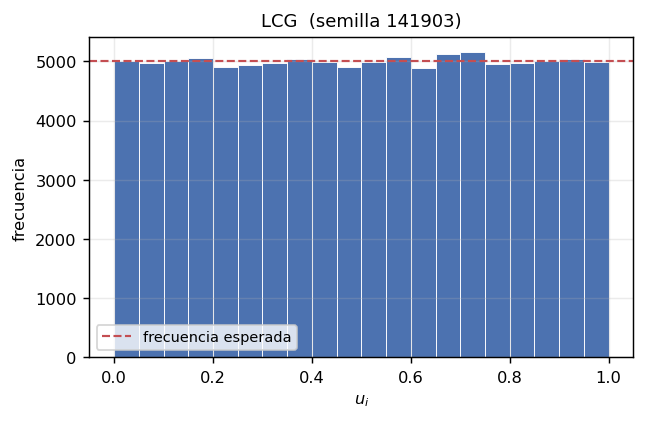
\includegraphics[width=0.62\textwidth]{hist_LCG.png}
\caption{Histograma de $N = \NMuestra$ valores del LCG con semilla
\Semilla, en $20$ celdas. La línea punteada marca la frecuencia esperada
bajo uniformidad.}
\label{fig:histLCG}
\end{figure}

% Generado por src/part1_generators.py.
% No editar a mano: se sobrescribe en cada ejecucion.
\begin{table}[htbp]\centering
\caption{Pruebas de hipotesis para LCG sobre $N=\NMuestra$ valores. Se rechaza $H_0$ al $5\%$ si $p<0.05$.}
\label{tab:pruebasLCG}
\small
\begin{tabular}{llrrl}
\toprule
Prueba & Mide & Estadistico & $p$-valor & Decision \\
\midrule
$\chi^2$ ($k=10$) & uniformidad & 6.17 & 0.7223 & no rechaza $H_0$ \\
Kolmogorov--Smirnov & uniformidad & 0.00312 & 0.2830 & no rechaza $H_0$ \\
Autocorrelacion lag-1 & independencia & +0.00119 & 0.7075 & no rechaza $H_0$ \\
Rachas & independencia & 49849 & 0.3364 & no rechaza $H_0$ \\
\bottomrule
\end{tabular}
\end{table}


En el histograma no hay ninguna celda que se despegue de la línea punteada, y
las cuatro pruebas dicen lo mismo. La chi-cuadrado da $X^2 = \statChiLCG$ con
$p = \pChiLCG$, lejísimos del umbral de $0.05$, así que no hay nada que
sugiera que las diez celdas se están apartando de lo esperado.
Kolmogorov--Smirnov da $D = \statKSLCG$ con $p = \pKSLCG$: la separación
máxima entre la acumulada empírica y la teórica anda en el orden de
$10^{-3}$, que es lo normal con $N = \NMuestra$. Del lado de la
independencia, la autocorrelación de retardo 1 sale $r_1 = \statLagLCG$ con
$p = \pLagLCG$, o sea indistinguible de cero, y la prueba de rachas cuenta
$R = \statRachasLCG$ rachas con $p = \pRachasLCG$, prácticamente el valor
esperado. Ninguna de las cuatro rechaza $H_0$, y este generador se porta
bien.

\begin{figure}[htbp]
\centering
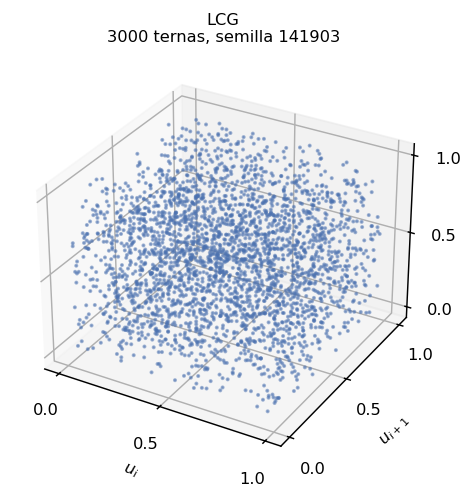
\includegraphics[width=0.46\textwidth]{cubo_LCG.png}
\caption{Ternas consecutivas $(u_i, u_{i+1}, u_{i+2})$ del LCG en el cubo
$[0,1]^3$ (\NTernas{} ternas).}
\label{fig:cuboLCG}
\end{figure}

En la figura~\ref{fig:cuboLCG} la nube llena el cubo y no se le ve ninguna
estructura. Ojo con la interpretación: eso no quiere decir que la retícula no
exista. Por la cota~\eqref{eq:marsaglia} sabemos que los planos están ahí,
pero al ser del orden de miles quedan separados por distancias de $10^{-3}$,
mucho más finas de lo que se puede distinguir en una figura con \NTernas{}
puntos. Comparado con RANDU (sección~\ref{sec:randu}), la diferencia es
puramente de cantidad: es el mismo tipo de defecto, sólo que tres órdenes de
magnitud más disimulado.

% ---------------------------------------------------------------------------
\subsection{Método de cuadrados medios (von Neumann)}

\subsubsection{Fundamento matemático}

Propuesto por von Neumann en 1949, es el primer PRNG de la historia. Se toma
un estado de $k$ dígitos decimales, se eleva al cuadrado para obtener hasta
$2k$ dígitos, se rellena con ceros a la izquierda hasta tener exactamente
$2k$, y se conservan los $k$ dígitos centrales:
\begin{equation}
X_{n+1} = \left\lfloor \frac{X_n^2}{10^{k/2}} \right\rfloor \bmod 10^{k},
\qquad U_n = \frac{X_n}{10^k}.
\label{eq:ms}
\end{equation}
La idea intuitiva es que los dígitos del centro de un cuadrado dependen de
todos los dígitos del original, así que ``mezclan'' bien.

\paragraph{Por qué aquí no hay ninguna garantía de período.} La diferencia de
fondo con el LCG es que el mapa~\eqref{eq:ms} \textbf{no es una biyección}.
Varios estados distintos pueden terminar con los mismos dígitos centrales, y
en cuanto eso pasa la órbita se va encogiendo. Un mapa cualquiera sobre un
conjunto de $n$ elementos arma lo que se llama un grafo funcional en forma de
$\rho$: una cola de estados que se visitan una sola vez y después un ciclo
del que ya no se sale nunca. Para un mapa tomado al azar, tanto la cola como
el ciclo miden en promedio del orden de $\sqrt{\pi n/8}$, o sea
$\mathcal{O}(10^{k/2})$ en vez del $10^k$ que uno esperaría viendo el tamaño
del espacio de estados. Se pierde la mitad de los dígitos de período nada más
por la forma que tiene el mapa.

\paragraph{Y encima el cero se traga todo.} Hay un modo de falla todavía
peor. Si en algún paso los dígitos centrales salen todos cero, entonces
$X_n = 0$, y como $0^2 = 0$ el generador se queda en cero para siempre. Es un
punto fijo sin salida: el generador no se vuelve periódico, se muere. Y hay
trampas parecidas, como los ciclos cortos de longitud 100 que aparecieron
probando otras semillas.

\paragraph{Lo que pasó con nuestra semilla.} Con $k = 8$ dígitos y semilla
\Semilla, la sucesión cae en el punto fijo $X = 0$ en el paso
$i = \CMColapso$, y el ciclo que queda tiene longitud \CMCiclo. Como la
muestra que pide la tarea es de $N = \NMuestra$ valores, resulta que el
\CMFracCeros{} de la muestra son ceros idénticos. Repitiendo el experimento
con 200 semillas consecutivas a partir de \Semilla, el tramo útil antes de
repetir un estado va de \CMLargoMin{} a \CMLargoMax{} pasos, con media
\CMLargoMedio. Esa dispersión gigante es justamente el punto: el método no
falla de manera predecible, falla distinto según la semilla que le toque, que
para un generador es lo peor de los dos mundos.

\subsubsection{Pseudocódigo}

\begin{pseudo}{Método de cuadrados medios}
\entrada{semilla $X_0$ de $k$ dígitos, con $k$ par; cantidad $N$.}
\salida{sucesión $u_1,\dots,u_N$ de valores en $[0,1)$.}
\begin{pasos}
  \item $X \gets X_0 \bmod 10^{k}$
  \item \textbf{para} $i = 1, 2, \dots, N$:
  \begin{pasos}
     \item $s \gets$ representación decimal de $X^2$, rellenada con ceros a la izquierda hasta $2k$ dígitos
     \item $X \gets$ el número formado por los $k$ dígitos centrales de $s$
     \item $u_i \gets X / 10^{k}$
     \item \textbf{si} $X = 0$: el generador degeneró y todo lo que sigue será cero
  \end{pasos}
  \item \textbf{devolver} $u_1, \dots, u_N$
\end{pasos}
\end{pseudo}

\subsubsection{Ficha comparativa}

\ficha{tab:fichaCM}{Características del método de cuadrados medios.}
{Alta en teoría, pero opera sobre la representación decimal, que obliga a
convertir a texto. Medido: \velCM{} valores por segundo.}
{Sin garantía alguna. Depende de la semilla y puede colapsar a cero. Con
semilla \Semilla{} el tramo útil fue de \CMColapso{} pasos.}
{Nula.}
{Sólo interés histórico y didáctico. Sirve justamente para mostrar por qué
hace falta una teoría de períodos antes de confiar en un generador.}

\subsubsection{Resultados de la implementación}

\begin{figure}[htbp]
\centering
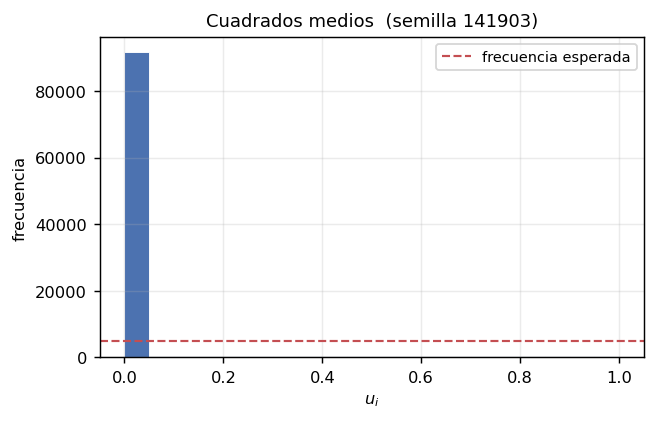
\includegraphics[width=0.62\textwidth]{hist_MiddleSquare.png}
\caption{Histograma de $N = \NMuestra$ valores del método de cuadrados
medios con semilla \Semilla. La barra de la primera celda se sale de la
escala: el \CMFracCeros{} de la muestra son ceros.}
\label{fig:histCM}
\end{figure}

% Generado por src/part1_generators.py.
% No editar a mano: se sobrescribe en cada ejecucion.
\begin{table}[htbp]\centering
\caption{Pruebas de hipotesis para Cuadrados medios sobre $N=\NMuestra$ valores. Se rechaza $H_0$ al $5\%$ si $p<0.05$.}
\label{tab:pruebasCM}
\small
\begin{tabular}{llrrl}
\toprule
Prueba & Mide & Estadistico & $p$-valor & Decision \\
\midrule
$\chi^2$ ($k=10$) & uniformidad & 748369.88 & $<10^{-12}$ & rechaza $H_0$ \\
Kolmogorov--Smirnov & uniformidad & 0.91138 & $<10^{-12}$ & rechaza $H_0$ \\
Autocorrelacion lag-1 & independencia & +0.73241 & $<10^{-12}$ & rechaza $H_0$ \\
Rachas & independencia & 0 & $<10^{-12}$ & rechaza $H_0$ \\
\bottomrule
\end{tabular}
\end{table}


Este histograma ni siquiera necesita estadística para leerse: casi toda la
masa está parada en el cero. Las cuatro pruebas rechazan $H_0$ de forma
catastrófica. La chi-cuadrado da $X^2 = \statChiCM$ contra un valor crítico
de $16.9$, cuatro órdenes de magnitud arriba. KS da $D = \statKSCM$, o sea que
la acumulada empírica se despega de la teórica casi tanto como es
matemáticamente posible, porque $D$ nunca puede pasar de 1. La
autocorrelación sale $r_1 = \statLagCM$, que era de esperarse: si la sucesión
es una constante, cada valor predice perfecto al siguiente. Y la prueba de
rachas cuenta $R = \statRachasCM$ rachas, sencillamente porque nunca se cruza
la mediana.

\begin{figure}[htbp]
\centering
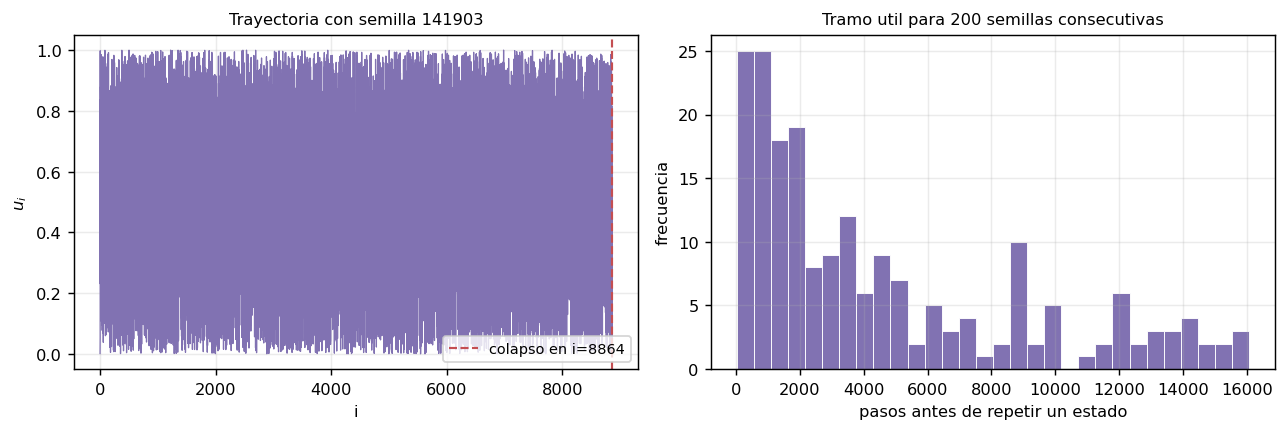
\includegraphics[width=\textwidth]{ms_colapso.png}
\caption{Izquierda: trayectoria del generador con semilla \Semilla; el
colapso al punto fijo cero ocurre en $i = \CMColapso$. Derecha: distribución
del largo del tramo útil para 200 semillas consecutivas.}
\label{fig:cm}
\end{figure}

Aquí hay que separar dos cosas que las pruebas están mezclando. Aplicadas a
los \NMuestra{} valores, lo que miden no es la calidad de los números sino el
colapso. Si en cambio se aplican sólo al tramo útil, o sea a los primeros
$n = \CMUtilN$ valores antes de que el generador se muera, el panorama cambia
por completo: $X^2 = \CMUtilChi$ con $p = \CMUtilChiP$ y $D = \CMUtilKS$ con
$p = \CMUtilKSP$, y ya no se rechaza $H_0$. Entonces la conclusión justa
sobre el método de von Neumann no es que produzca números mal distribuidos,
sino que produce pocos. Mientras dura se ve bastante decente; el problema es
que se acaba.

% ---------------------------------------------------------------------------
\subsection{Mersenne Twister (MT19937)}
\label{sec:mt}

\subsubsection{Fundamento matemático}

MT19937 (Matsumoto y Nishimura, 1998) es el generador estándar de Python, R,
MATLAB y NumPy. Es un \emph{generador de Fibonacci retardado torcido}, y toda
su teoría vive en el cuerpo $\mathbb{F}_2 = \{0,1\}$: cada palabra de $32$
bits se ve como un vector de $\mathbb{F}_2^{32}$ y todas las operaciones
(\textsc{xor}, desplazamientos, máscaras) son lineales sobre ese cuerpo.

\paragraph{La recurrencia.} El estado son $n = 624$ palabras de $w = 32$
bits. La recurrencia combina dos palabras separadas por $m = 397$ posiciones:
\begin{equation}
\mathbf{x}_{k+n} = \mathbf{x}_{k+m} \oplus
\left( (\mathbf{x}_k^{u} \mid \mathbf{x}_{k+1}^{l})\, A \right),
\label{eq:mt}
\end{equation}
donde $\mathbf{x}_k^{u}$ es el bit más significativo de $\mathbf{x}_k$,
$\mathbf{x}_{k+1}^{l}$ son los $31$ bits menos significativos de
$\mathbf{x}_{k+1}$, la barra vertical los concatena en una palabra de 32
bits, y $A$ es la matriz compañera de $32\times32$ cuya acción se calcula sin
multiplicar matrices:
\begin{equation}
\mathbf{y} A =
\begin{cases}
\mathbf{y} \gg 1 & \text{si el bit menos significativo de } \mathbf{y}
\text{ es } 0,\\[2pt]
(\mathbf{y} \gg 1) \oplus \texttt{0x9908B0DF} & \text{en otro caso.}
\end{cases}
\end{equation}
El nombre ``torcido'' viene precisamente de esa matriz $A$, que es la
torsión que rompe la simetría del retardo de Fibonacci.

\paragraph{De dónde sale el período.} Toda la iteración es una aplicación
lineal $\mathbf{s} \mapsto B\mathbf{s}$ sobre el espacio de estados
$\mathbb{F}_2^{nw - r}$, donde $r = 31$ son los bits que se descartan de la
primera palabra. La dimensión efectiva es
\begin{equation}
nw - r = 624 \times 32 - 31 = 19937.
\end{equation}
El período del generador es el orden de $B$ en el grupo lineal, y ese orden
es $2^{19937}-1$ si y sólo si el polinomio característico de $B$ es
\emph{primitivo} sobre $\mathbb{F}_2$. Los autores eligieron los parámetros
$(n, m, r, a)$ justamente para que lo fuera, verificándolo con la
factorización conocida de $2^{19937}-1$, que es un primo de Mersenne: de ahí
el nombre del generador. Que el número sea primo ayuda, porque entonces
cualquier estado no nulo tiene automáticamente período completo.

\paragraph{Templado.} La salida cruda de la recurrencia no se entrega
directamente. Pasa antes por un \emph{templado} (\emph{tempering}), que es
otra transformación lineal invertible sobre $\mathbb{F}_2^{32}$:
\begin{align}
y &\gets y \oplus (y \gg 11), &
y &\gets y \oplus ((y \ll 7)\ \&\ \texttt{0x9D2C5680}),\\
y &\gets y \oplus ((y \ll 15)\ \&\ \texttt{0xEFC60000}), &
y &\gets y \oplus (y \gg 18).
\end{align}
El templado no cambia el período, porque es invertible; lo que hace es
mejorar la equidistribución de los bits individuales.

\paragraph{Equidistribución.} Ésta es la propiedad que de verdad importa y
que separa a MT19937 de todo lo anterior. El generador es
\emph{equidistribuido a 32 bits de precisión en 623 dimensiones}: si se toman
las $623$-tuplas consecutivas de salidas y se miran sus $32$ bits, cada
patrón posible aparece el mismo número de veces en un período completo
(salvo el caso del cero). Es decir, la retícula que en el LCG se veía en
dimensión 3 aquí no aparece hasta después de la dimensión 623. Por eso pasa
la prueba espectral en las dimensiones donde RANDU se hunde.

\paragraph{Lo que no es.} Con todo lo bueno que tiene, MT19937 no sirve para
criptografía. Como toda la recurrencia es lineal, a alguien le basta con ver
624 salidas seguidas para invertir el templado, reconstruir el estado
completo y predecir todo lo que viene después. Es rapidísimo y
estadísticamente impecable, pero completamente predecible si uno lo mira con
las herramientas correctas.

\subsubsection{Pseudocódigo}

\begin{pseudo}{Mersenne Twister MT19937}
\entrada{semilla $s$; cantidad $N$. Constantes $n=624$, $m=397$,
$A = \texttt{0x9908B0DF}$.}
\salida{sucesión $u_1,\dots,u_N$ de valores en $[0,1)$.}
\begin{pasos}
  \item \textbf{Inicialización del estado:}
  \begin{pasos}
     \item $mt[0] \gets s \bmod 2^{32}$
     \item \textbf{para} $i = 1, \dots, n-1$:
       $mt[i] \gets \big(1812433253 \cdot (mt[i-1] \oplus (mt[i-1] \gg 30)) + i\big) \bmod 2^{32}$
     \item $\textit{idx} \gets n$ \quad \textcolor{gris}{\small(fuerza una torsión en la primera llamada)}
  \end{pasos}
  \item \textbf{para} $i = 1, \dots, N$:
  \begin{pasos}
     \item \textbf{si} $\textit{idx} \ge n$, aplicar la torsión a todo el estado:
     \begin{pasos}
        \item \textbf{para} $j = 0, \dots, n-1$:
        \item \quad $y \gets (mt[j]\ \&\ \texttt{0x80000000})\ |\ (mt[(j+1) \bmod n]\ \&\ \texttt{0x7FFFFFFF})$
        \item \quad $mt[j] \gets mt[(j+m) \bmod n] \oplus (y \gg 1)$
        \item \quad \textbf{si} $y$ es impar: $mt[j] \gets mt[j] \oplus A$
        \item $\textit{idx} \gets 0$
     \end{pasos}
     \item $y \gets mt[\textit{idx}]$; \quad $\textit{idx} \gets \textit{idx} + 1$
     \item Templado: $y \gets y \oplus (y \gg 11)$; \quad
           $y \gets y \oplus ((y \ll 7)\ \&\ \texttt{0x9D2C5680})$; \quad
           $y \gets y \oplus ((y \ll 15)\ \&\ \texttt{0xEFC60000})$; \quad
           $y \gets y \oplus (y \gg 18)$
     \item $u_i \gets y / 2^{32}$
  \end{pasos}
  \item \textbf{devolver} $u_1, \dots, u_N$
\end{pasos}
\end{pseudo}

\subsubsection{Ficha comparativa}

\ficha{tab:fichaMT}{Características del Mersenne Twister.}
{Media. El estado de 624 palabras se recalcula por bloques, así que una de
cada 624 llamadas es cara y las demás son baratas. Medido: \velMT{} valores
por segundo en Python puro; la versión en C de \code{random} es más de 20
veces más rápida.}
{$2^{19937}-1$, garantizado por la primitividad del polinomio
característico. Para efectos prácticos, inagotable.}
{Nula. Con 624 salidas consecutivas se invierte el templado y se reconstruye
el estado completo.}
{Estándar de facto en simulación científica y estadística: Python, R,
MATLAB, NumPy. Es la opción correcta por defecto cuando no se necesita
seguridad criptográfica.}

\subsubsection{Resultados de la implementación}

\begin{figure}[htbp]
\centering
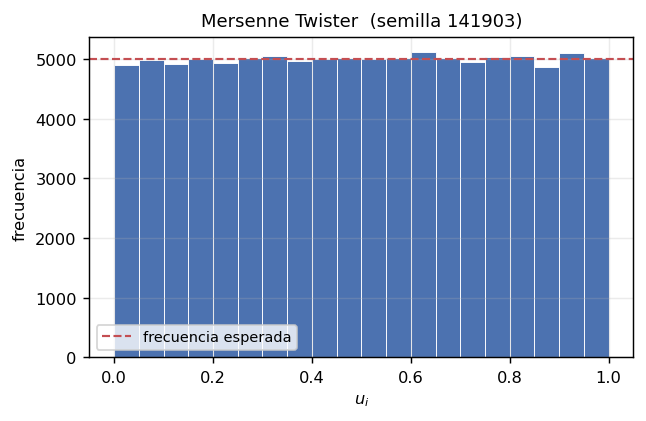
\includegraphics[width=0.62\textwidth]{hist_MersenneTwister.png}
\caption{Histograma de $N = \NMuestra$ valores de la implementación propia de
MT19937 con semilla \Semilla.}
\label{fig:histMT}
\end{figure}

% Generado por src/part1_generators.py.
% No editar a mano: se sobrescribe en cada ejecucion.
\begin{table}[htbp]\centering
\caption{Pruebas de hipotesis para Mersenne Twister sobre $N=\NMuestra$ valores. Se rechaza $H_0$ al $5\%$ si $p<0.05$.}
\label{tab:pruebasMT}
\small
\begin{tabular}{llrrl}
\toprule
Prueba & Mide & Estadistico & $p$-valor & Decision \\
\midrule
$\chi^2$ ($k=10$) & uniformidad & 6.51 & 0.6879 & no rechaza $H_0$ \\
Kolmogorov--Smirnov & uniformidad & 0.00303 & 0.3175 & no rechaza $H_0$ \\
Autocorrelacion lag-1 & independencia & +0.00245 & 0.4393 & no rechaza $H_0$ \\
Rachas & independencia & 49904 & 0.5396 & no rechaza $H_0$ \\
\bottomrule
\end{tabular}
\end{table}


Las cuatro pruebas salen como uno esperaría del generador que todo el mundo
usa de referencia. La chi-cuadrado da $X^2 = \statChiMT$ con $p = \pChiMT$ y
KS da $D = \statKSMT$ con $p = \pKSMT$, así que la muestra es indistinguible
de una uniforme de verdad. En independencia, $r_1 = \statLagMT$ con
$p = \pLagMT$ y $R = \statRachasMT$ rachas con $p = \pRachasMT$. Ninguna
rechaza $H_0$. Y un detalle que vale la pena notar: los $p$-valores tampoco
son sospechosamente altos, porque eso también sería mala señal; un $p$ casi
igual a 1 significaría que los datos se ajustan \emph{demasiado} bien a la
uniforme, que es lo que pasa cuando alguien los acomodó.

\paragraph{Validación de la implementación.} Una implementación propia de
MT19937 se puede verificar de manera mucho más fuerte que con pruebas
estadísticas, porque el algoritmo es determinista y está publicado:
\begin{enumerate}[itemsep=2pt]
  \item Con la semilla oficial $5489$, las primeras salidas de 32 bits son
        $3499211612$, $581869302$, $3890346734$, $3586334585$, $545404204$,
        que coinciden con el vector de referencia de los autores.
  \item Implementando además el sembrado \code{init\_by\_array} que usa
        CPython y el empaquetado de 53 bits de \code{genrand\_res53}, la
        implementación propia reproduce \textbf{bit a bit} la salida de
        \code{random.random()} para la misma semilla. La verificación
        automática sobre \NMuestra{} valores da: idéntico = \MTIdentico.
\end{enumerate}

\begin{figure}[htbp]
\centering
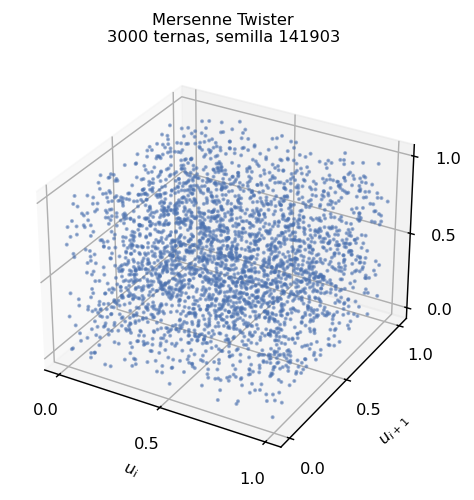
\includegraphics[width=0.46\textwidth]{cubo_MersenneTwister.png}
\caption{Ternas consecutivas del Mersenne Twister en el cubo $[0,1]^3$.}
\label{fig:cuboMT}
\end{figure}

La nube de ternas de la figura~\ref{fig:cuboMT} no muestra estructura, y en
este caso sabemos que no la hay hasta dimensión 623, no sólo que no se ve.

\paragraph{Comparación con \code{random} y \code{secrets}.} El generador
elegido para el inciso (d) es este mismo. Las tres fuentes comparadas son:
\begin{itemize}[itemsep=2pt]
  \item la implementación propia de MT19937;
  \item \code{random}, que es exactamente el mismo algoritmo implementado en
        C dentro de CPython. Es reproducible a partir de una semilla y no
        sirve para criptografía;
  \item \code{secrets}, que es la interfaz al generador criptográfico del
        sistema operativo (\code{/dev/urandom} en Linux). No acepta semilla y
        no es reproducible, precisamente porque su propósito es que nadie
        pueda predecir su salida.
\end{itemize}

\begin{figure}[htbp]
\centering
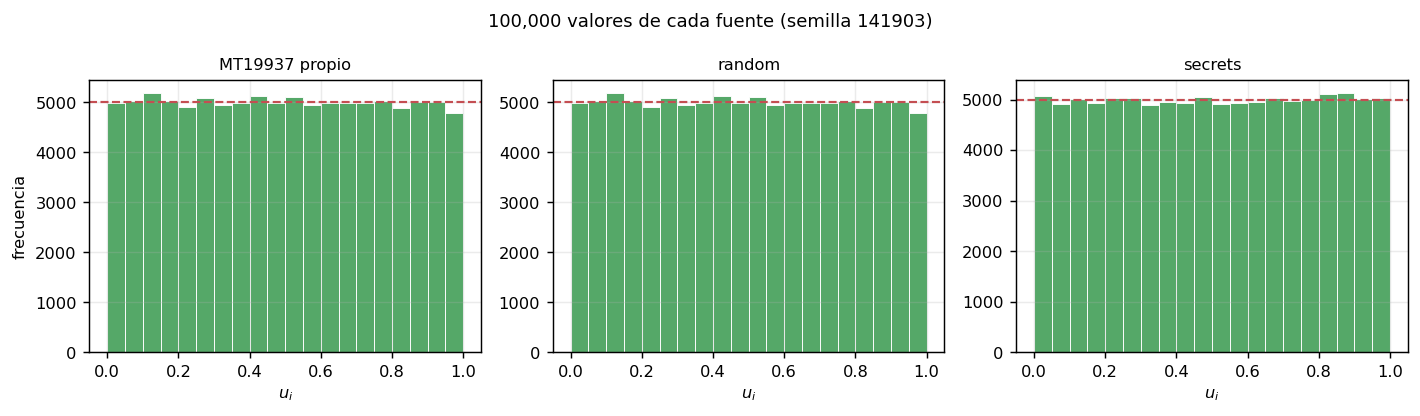
\includegraphics[width=\textwidth]{comparacion_librerias.png}
\caption{Histogramas de $N = \NMuestra$ valores de las tres fuentes.}
\label{fig:libs}
\end{figure}

% Generado por src/part1_generators.py.
% No editar a mano: se sobrescribe en cada ejecucion.
\begin{table}[htbp]\centering
\caption{MT19937 propio frente a \texttt{random} y \texttt{secrets} ($N=\NMuestra$).}
\label{tab:librerias}
\small
\begin{tabular}{lrrrrr}
\toprule
Fuente & Valores/s & $X^2$ & $p_{\chi^2}$ & $D$ & $p_{KS}$ \\
\midrule
\texttt{MT19937 propio} & 459{,}593 & 11.71 & 0.2300 & 0.00381 & 0.1092 \\
\texttt{random} & 15{,}382{,}116 & 11.71 & 0.2300 & 0.00381 & 0.1092 \\
\texttt{secrets} & 1{,}174{,}510 & 9.34 & 0.4066 & 0.00205 & 0.7965 \\
\bottomrule
\end{tabular}
\end{table}


De la tabla~\ref{tab:librerias} salen tres lecturas. La primera es que las
tres fuentes son estadísticamente equivalentes: todos los $p$-valores de
$\chi^2$ y KS están muy por encima de $0.05$, y entre la implementación
propia y \code{random} los estadísticos coinciden \emph{exactamente}, lo cual
no es coincidencia sino la consecuencia de que son literalmente los mismos
números. La segunda es que la diferencia de velocidad pasa del orden de
magnitud, y eso es puro costo de Python interpretado contra C, porque el
algoritmo es idéntico: sirve para recordar que ``lento'' casi nunca es
propiedad del algoritmo sino de cómo está escrito. Y la tercera es que
\code{secrets} sale más lento que \code{random} y encima no es reproducible,
así que para simulación es la peor de las tres. Suena contraintuitivo que el
generador más seguro sea el peor para esto, pero tiene sentido: en simulación
uno quiere poder repetir el experimento con la misma semilla, y eso es
justamente lo que un generador criptográfico está diseñado para impedir.

% ---------------------------------------------------------------------------
\subsection{Blum Blum Shub}

\subsubsection{Fundamento matemático}

BBS (Blum, Blum y Shub, 1986) es de una familia distinta: es un generador
\emph{criptográficamente seguro}, y su diseño no busca velocidad sino una
garantía demostrable. Se toma $N = pq$ con $p$ y $q$ primos distintos tales
que
\begin{equation}
p \equiv q \equiv 3 \pmod 4,
\end{equation}
lo que hace de $N$ un \emph{entero de Blum}, y se itera el cuadrado modular
\begin{equation}
x_{n+1} = x_n^2 \bmod N,
\label{eq:bbs}
\end{equation}
extrayendo en cada paso los $j$ bits menos significativos de $x_n$, con
$j = \lfloor \log_2 \log_2 N \rfloor$.

\paragraph{Por qué los primos tienen que ser congruentes con 3 módulo 4.}
Sea $QR_N$ el conjunto de residuos
cuadráticos módulo $N$. Cuando $p \equiv 3 \pmod 4$, exactamente una de las
dos raíces cuadradas de un residuo cuadrático módulo $p$ es a su vez un
residuo cuadrático; esa raíz se llama la raíz principal. Con la misma
condición sobre $q$, el mapa $x \mapsto x^2$ resulta ser una
\emph{permutación} de $QR_N$. Esto es lo que garantiza que la órbita sea un
ciclo puro, sin cola: no hay estados que se visiten una sola vez y el
generador nunca se degrada como los cuadrados medios.

\paragraph{Seguridad.} Predecir el siguiente bit de salida con ventaja no
despreciable sobre el volado es tan difícil como decidir residuosidad
cuadrática módulo $N$, problema que se cree tan difícil como factorizar $N$.
Ésta es la diferencia cualitativa con todos los generadores anteriores: la
seguridad no es una observación empírica, es una reducción. Sacar
$j = \lfloor \log_2\log_2 N\rfloor$ bits por paso, y no más, es parte del
teorema: es la cantidad de bits que se puede extraer sin debilitar la
reducción.

\paragraph{Un error que valió la pena cometer.} Aquí hay algo que al
principio parecía un bug del código y terminó siendo teoría: la condición
$p \equiv q \equiv 3 \pmod 4$ es necesaria pero \textbf{no suficiente} para
tener buen período. El período de la órbita de~\eqref{eq:bbs} es
\begin{equation}
\ord_{\lambda(\lambda(N))}(2),
\end{equation}
el orden multiplicativo de $2$ módulo $\lambda(\lambda(N))$, donde $\lambda$
es la función de Carmichael. La razón es que
$x_n = x_0^{2^n} \bmod N$, de modo que el exponente $2^n$ vive módulo
$\lambda(N)$ y el período se reduce a preguntar cuándo $2^n$ se repite ahí.

En el primer intento usé los primos de Mersenne $p = 2^{31}-1$ y
$q = 2^{61}-1$, que sí cumplen lo de $3 \bmod 4$ y además son famosos, así
que parecían una buena idea. El generador colapsó a un ciclo de unos 30
estados: de los 64 valores posibles de un bloque de 6 bits sólo aparecían 44,
y las pruebas de uniformidad rechazaban $H_0$ por goleada. La causa es que
$p-1$ y $q-1$ se factorizan en primos chiquitos, entonces
$\lambda(\lambda(N))$ queda pequeño y el orden de 2 también. Ser primo no
alcanza: importa cómo se factoriza el número de al lado.

La solución es exigir \emph{primos seguros}, es decir $p = 2p'+1$ con $p'$
también primo, lo que obliga a $\lambda(N)$ a tener un factor primo grande.
La implementación final usa
\[
p = 4294967387 = 2 \cdot 2147483693 + 1, \qquad
q = 8589935363 = 2 \cdot 4294967681 + 1,
\]
ambos primos seguros y congruentes con $3 \bmod 4$. Con esos parámetros el
generador pasa las cuatro pruebas.

\subsubsection{Pseudocódigo}

\begin{pseudo}{Blum Blum Shub}
\entrada{primos seguros $p \equiv q \equiv 3 \pmod 4$; semilla $s$ coprima
con $N = pq$ y distinta de $0$ y $1$; cantidad $N_{\text{out}}$ de valores;
ancho de salida $w = 32$ bits.}
\salida{sucesión $u_1,\dots,u_{N_{\text{out}}}$ de valores en $[0,1)$.}
\begin{pasos}
  \item $N \gets p \cdot q$; \quad $j \gets \lfloor \log_2 \log_2 N \rfloor$
  \item Verificar que $\mcd(s, N) = 1$; si no, la semilla es inválida.
  \item $x \gets s^2 \bmod N$ \quad \textcolor{gris}{\small(entra al conjunto de residuos cuadráticos)}
  \item \textbf{para} $i = 1, \dots, N_{\text{out}}$:
  \begin{pasos}
     \item $v \gets 0$; \quad $b \gets 0$
     \item \textbf{mientras} $b < w$:
     \begin{pasos}
       \item $x \gets x^2 \bmod N$
       \item $t \gets \min(j,\ w - b)$ \quad \textcolor{gris}{\small(no tomar más bits de los que faltan)}
       \item $v \gets (v \ll t)\ |\ (x\ \&\ (2^{t}-1))$
       \item $b \gets b + t$
     \end{pasos}
     \item $u_i \gets v / 2^{w}$
  \end{pasos}
  \item \textbf{devolver} $u_1, \dots, u_{N_{\text{out}}}$
\end{pasos}
\end{pseudo}

\subsubsection{Ficha comparativa}

\ficha{tab:fichaBBS}{Características de Blum Blum Shub.}
{Muy baja. Cada bloque de $j$ bits cuesta una multiplicación modular sobre
enteros de 66 bits, así que un solo valor de 32 bits requiere varias. Medido:
\velBBS{} valores por segundo, unas diez veces menos que el LCG.}
{Es $\ord_{\lambda(\lambda(N))}(2)$ y depende finamente de $p$ y $q$: con
primos mal elegidos puede ser de unas decenas de estados, con primos seguros
es astronómico.}
{Demostrable. Predecir la salida equivale a resolver el problema de la
residuosidad cuadrática, que se cree tan difícil como factorizar $N$. Es el
único de los cinco con una garantía de este tipo.}
{Criptografía: generación de claves y \emph{nonces}, cuando el costo por bit
se puede tolerar. Nunca para simulación masiva.}

\subsubsection{Resultados de la implementación}

\begin{figure}[htbp]
\centering
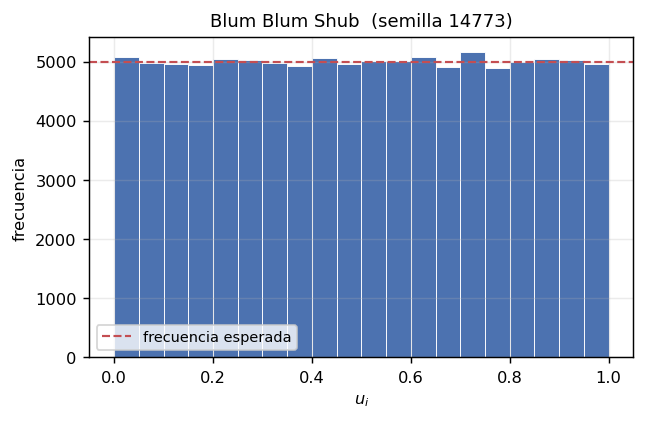
\includegraphics[width=0.62\textwidth]{hist_BlumBlumShub.png}
\caption{Histograma de $N = \NMuestra$ valores de Blum Blum Shub con semilla
\SemillaBBS.}
\label{fig:histBBS}
\end{figure}

% Generado por src/part1_generators.py.
% No editar a mano: se sobrescribe en cada ejecucion.
\begin{table}[htbp]\centering
\caption{Pruebas de hipotesis para Blum Blum Shub sobre $N=\NMuestra$ valores. Se rechaza $H_0$ al $5\%$ si $p<0.05$.}
\label{tab:pruebasBBS}
\small
\begin{tabular}{llrrl}
\toprule
Prueba & Mide & Estadistico & $p$-valor & Decision \\
\midrule
$\chi^2$ ($k=10$) & uniformidad & 3.27 & 0.9527 & no rechaza $H_0$ \\
Kolmogorov--Smirnov & uniformidad & 0.00132 & 0.9948 & no rechaza $H_0$ \\
Autocorrelacion lag-1 & independencia & +0.00048 & 0.8786 & no rechaza $H_0$ \\
Rachas & independencia & 49993 & 0.9596 & no rechaza $H_0$ \\
\bottomrule
\end{tabular}
\end{table}


Ya con los primos seguros, el generador se porta muy bien: $X^2 =
\statChiBBS$ con $p = \pChiBBS$ y $D = \statKSBBS$ con $p = \pKSBBS$ del lado
de la uniformidad, y $r_1 = \statLagBBS$ con $p = \pLagBBS$ más
$R = \statRachasBBS$ rachas con $p = \pRachasBBS$ del lado de la
independencia. Ninguna de las cuatro rechaza $H_0$. Lo más interesante de
esta tabla es lo que no se ve: estos mismos números, con los
primos de Mersenne del primer intento, rechazaban $H_0$ en las cuatro
pruebas. El código era idéntico, lo único que cambió fueron dos constantes.
En criptografía los parámetros no son configuración, son parte del algoritmo.

% ---------------------------------------------------------------------------
\subsection{RANDU}
\label{sec:randu}

\subsubsection{Fundamento matemático}

RANDU es el LCG multiplicativo que IBM distribuyó en los años 60 dentro de su
System/360 y que se usó durante más de una década en trabajo científico:
\begin{equation}
X_{n+1} = 65539\, X_n \bmod 2^{31},
\qquad X_0 \text{ impar}.
\label{eq:randudef}
\end{equation}
La elección parece razonable a primera vista: $a = 65539 = 2^{16}+3$ permite
calcular la multiplicación con un desplazamiento y dos sumas, que en hardware
de los años 60 era una ventaja real.

\paragraph{Período.} Como $c = 0$, no aplica Hull--Dobell. Para un generador
multiplicativo con $m = 2^{31}$, el estado nunca puede ser par si la semilla
es impar (multiplicar impares da impar), así que la órbita vive en un
subconjunto. El período máximo posible es $m/4 = 2^{29}$ y RANDU lo alcanza.
Ya de entrada es un período cuatro veces menor que el de un LCG mixto con el
mismo módulo, pero ése no es el problema serio.

\paragraph{El defecto fatal.} El problema es algebraico y exacto. Escribiendo
$a = 65539 = 2^{16}+3$:
\begin{align}
a^2 &= (2^{16}+3)^2 = 2^{32} + 6\cdot 2^{16} + 9 \nonumber\\
    &= 6\,(2^{16}+3) - 9 + 2^{32} \nonumber\\
    &\equiv 6a - 9 \pmod{2^{31}},
\end{align}
donde el término $2^{32}$ desaparece porque es múltiplo de $2^{31}$.
Multiplicando la relación $a^2 \equiv 6a - 9$ por $X_n$ se obtiene, para todo
$n$,
\begin{equation}
\boxed{\,X_{n+2} = 6 X_{n+1} - 9 X_n \pmod{2^{31}}\,}
\label{eq:randu}
\end{equation}
Es decir, cada valor es una combinación lineal entera exacta de los dos
anteriores. Dividiendo entre $2^{31}$, las ternas normalizadas satisfacen
\begin{equation}
9 u_n - 6 u_{n+1} + u_{n+2} = k, \qquad k \in \mathbb{Z}.
\label{eq:randuplanos}
\end{equation}

\paragraph{Cuántos planos.} La ecuación~\eqref{eq:randuplanos} dice que toda
terna consecutiva cae en alguno de los planos paralelos de vector normal
$(9,-6,1)$. Como cada $u \in [0,1)$, la combinación $9u_n - 6u_{n+1}+u_{n+2}$
está acotada entre $-6$ y $10$, y sólo puede tomar los valores enteros en ese
rango: exactamente \PlanosRandu{} planos. La cota de Marsaglia
\eqref{eq:marsaglia} para $m = 2^{31}$ y $d = 3$ permitiría hasta
$(6\cdot 2^{31})^{1/3} \approx 2344$ planos, así que RANDU aprovecha menos
del uno por ciento de la estructura que su módulo le permitiría. Esto es lo
que Marsaglia bautizó como ``los números aleatorios caen principalmente en
los planos'' \cite{marsaglia1968}.

\subsubsection{Pseudocódigo}

\begin{pseudo}{RANDU}
\entrada{semilla impar $X_0$; cantidad $N$.}
\salida{sucesión $u_1,\dots,u_N$ de valores en $[0,1)$.}
\begin{pasos}
  \item Verificar que $X_0$ sea impar; si es par, la órbita se degrada.
  \item $X \gets X_0 \bmod 2^{31}$
  \item \textbf{para} $i = 1, \dots, N$:
  \begin{pasos}
     \item $X \gets 65539 \cdot X \bmod 2^{31}$
     \item $u_i \gets X / 2^{31}$
  \end{pasos}
  \item \textbf{devolver} $u_1, \dots, u_N$
\end{pasos}
\end{pseudo}

\subsubsection{Ficha comparativa}

\ficha{tab:fichaRANDU}{Características de RANDU.}
{Muy alta. Una multiplicación y un módulo por valor, y la multiplicación se
puede hacer con desplazamientos. Medido: \velRANDU{} valores por segundo, el
más rápido de los cinco.}
{$2^{29}$ con semilla impar, la cuarta parte del módulo.}
{Nula, y además con una relación lineal explícita entre términos
consecutivos que permite predecir la sucesión con sólo dos valores.}
{Ninguno. Es el contraejemplo canónico de mal diseño y sólo se usa hoy con
fines didácticos, como aquí.}

\subsubsection{Resultados de la implementación}

\begin{figure}[htbp]
\centering
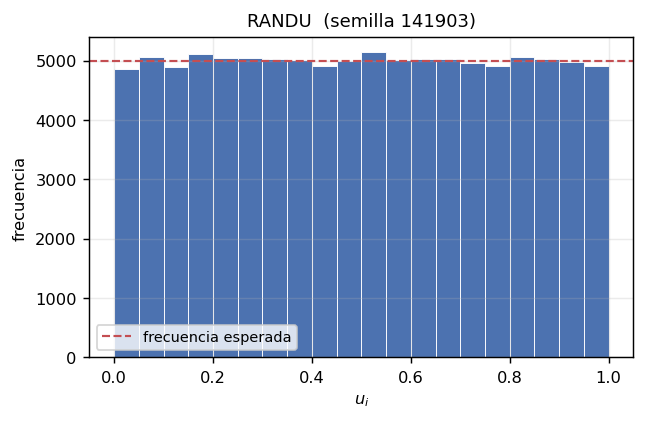
\includegraphics[width=0.62\textwidth]{hist_RANDU.png}
\caption{Histograma de $N = \NMuestra$ valores de RANDU con semilla
\Semilla.}
\label{fig:histRANDU}
\end{figure}

% Generado por src/part1_generators.py.
% No editar a mano: se sobrescribe en cada ejecucion.
\begin{table}[htbp]\centering
\caption{Pruebas de hipotesis para RANDU sobre $N=\NMuestra$ valores. Se rechaza $H_0$ al $5\%$ si $p<0.05$.}
\label{tab:pruebasRANDU}
\small
\begin{tabular}{llrrl}
\toprule
Prueba & Mide & Estadistico & $p$-valor & Decision \\
\midrule
$\chi^2$ ($k=10$) & uniformidad & 8.80 & 0.4561 & no rechaza $H_0$ \\
Kolmogorov--Smirnov & uniformidad & 0.00220 & 0.7185 & no rechaza $H_0$ \\
Autocorrelacion lag-1 & independencia & -0.00024 & 0.9390 & no rechaza $H_0$ \\
Rachas & independencia & 50136 & 0.3932 & no rechaza $H_0$ \\
\bottomrule
\end{tabular}
\end{table}


Y aquí está el punto central de toda la Parte 1. RANDU \textbf{pasa las
cuatro pruebas}: $X^2 = \statChiRANDU$ con $p = \pChiRANDU$,
$D = \statKSRANDU$ con $p = \pKSRANDU$, $r_1 = \statLagRANDU$ con
$p = \pLagRANDU$ y $R = \statRachasRANDU$ rachas con $p = \pRachasRANDU$.
Si uno se quedara con esta tabla, tendría que concluir que RANDU está al
nivel del Mersenne Twister, lo cual sabemos que es falso.

Y no es que a las pruebas les haya faltado potencia estadística, ni que $N$
sea chico. El problema es estructural: chi-cuadrado y KS miran un valor a la
vez, la autocorrelación y las rachas miran parejas, y el defecto de RANDU
vive en las \emph{ternas}. Ninguna de las cuatro mira ternas, así que no hay
forma de que lo encuentren. Subir $N$ a mil millones tampoco serviría de
nada; lo que hay que cambiar es la herramienta, no el tamaño de la muestra.

\begin{figure}[htbp]
\centering
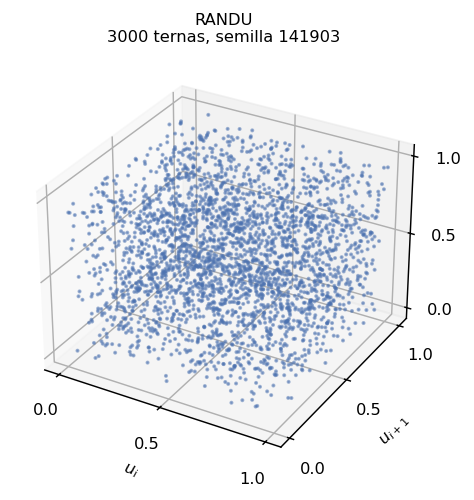
\includegraphics[width=0.46\textwidth]{cubo_RANDU.png}
\caption{Ternas consecutivas de RANDU vistas desde un ángulo arbitrario.
Comparar con las figuras~\ref{fig:cuboLCG} y~\ref{fig:cuboMT}: desde aquí
los tres generadores se ven igual de aceptables.}
\label{fig:cuboRANDU}
\end{figure}

\begin{figure}[htbp]
\centering
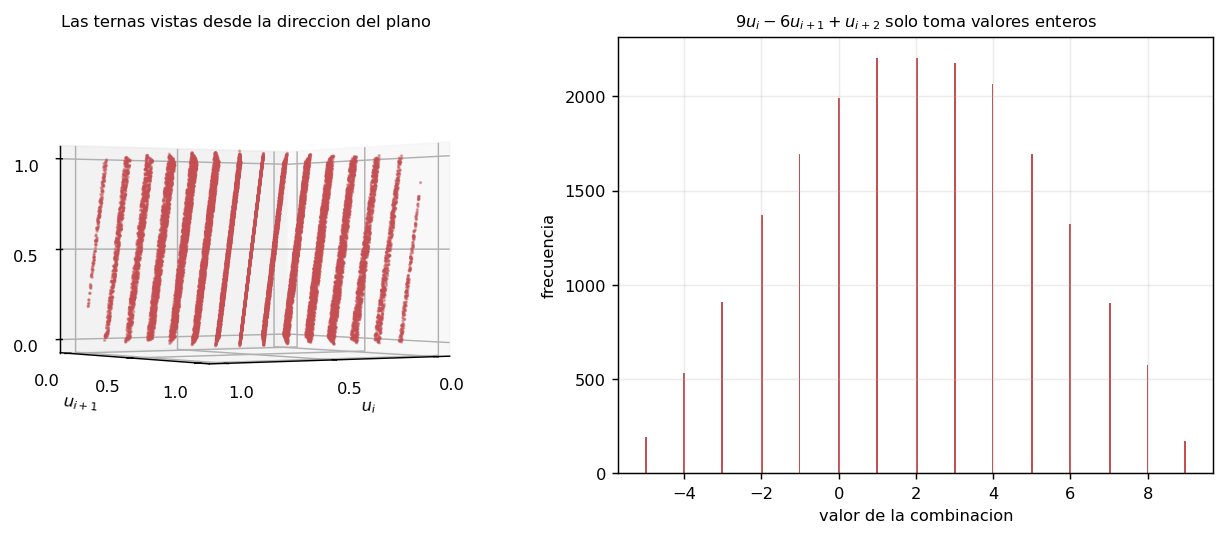
\includegraphics[width=\textwidth]{randu_planos.png}
\caption{Izquierda: las mismas ternas vistas desde una dirección
perpendicular al vector normal $(9,-6,1)$; los \PlanosRandu{} planos aparecen
de canto. Derecha: la combinación $9u_i - 6u_{i+1} + u_{i+2}$ sólo toma
\PlanosRandu{} valores enteros distintos, con residuo máximo a entero de
\ResiduoRandu.}
\label{fig:planos}
\end{figure}

La figura~\ref{fig:cuboRANDU} está puesta ahí a propósito para engañar:
mirada desde un ángulo cualquiera, la nube de RANDU se ve igual de llena que
la del LCG o la del Mersenne Twister. La figura~\ref{fig:planos} es
exactamente la misma nube, sólo que girada hasta quedar mirando en la
dirección del vector normal $(9,-6,1)$, y de repente todo el volumen se
aplasta en \PlanosRandu{} láminas. El panel de la derecha lo confirma sin
lugar a dudas: la combinación de la ecuación~\eqref{eq:randuplanos} toma
exactamente \PlanosRandu{} valores enteros, con un residuo máximo de
\ResiduoRandu, o sea cero hasta donde la máquina puede medir. Esto no es una
tendencia estadística que uno podría discutir, es una identidad algebraica.

De aquí salen dos cosas. La primera es que el defecto no aparece solo:
hay que saber qué buscar, y quien dice dónde mirar es el álgebra de la
ecuación~\eqref{eq:randu}, no los datos. Si uno se limita a graficar desde el
ángulo por defecto, no encuentra nada. La segunda es que todo LCG tiene esta
misma estructura, incluido el de la sección anterior; la diferencia es que
uno bien parametrizado reparte sus ternas entre miles de planos pegaditos y
RANDU las reparte entre \PlanosRandu{} planos separados por huecos enormes.
Y eso conecta con el período de una forma que vale la pena decir explícito:
RANDU produce $2^{29}$ valores distintos, que no es poco, pero la calidad no
se mide sólo por cuántos números salen antes de repetirse, sino por cómo se
acomodan en el espacio donde uno los va a usar. En la Parte 2 se ve qué le
pasa a un cálculo de Monte Carlo en tres dimensiones cuando lo alimenta este
generador.

% ---------------------------------------------------------------------------
\subsection{Comparación global de los cinco generadores}

\begin{table}[htbp]
\centering
\caption{Resumen comparativo. Las velocidades son las medidas en Python puro
(tabla~\ref{tab:velocidad}).}
\label{tab:comparativa}
\scriptsize
\begin{tabular}{p{2.1cm}p{2.5cm}p{2.9cm}p{2.7cm}p{3.6cm}}
\toprule
Algoritmo & Velocidad & Período & Seguridad & Casos de uso \\
\midrule
LCG &
Muy alta (\velLCG/s) &
$2^{32}$ por Hull--Dobell &
Nula: el estado se recupera con pocas salidas &
Simulación no crítica, videojuegos, sistemas embebidos \\
\addlinespace
Cuadrados medios &
Alta (\velCM/s) &
Sin garantía; degenera. Aquí \CMColapso{} pasos &
Nula &
Sólo interés histórico y didáctico \\
\addlinespace
Mersenne Twister &
Media (\velMT/s) &
$2^{19937}-1$ &
Nula: 624 salidas bastan para reconstruir el estado &
Estándar en simulación científica: Python, R, MATLAB, NumPy \\
\addlinespace
Blum Blum Shub &
Muy baja (\velBBS/s) &
$\ord_{\lambda(\lambda(N))}(2)$; exige primos seguros &
Demostrable: equivale a factorizar $N$ &
Criptografía: claves y \emph{nonces} \\
\addlinespace
RANDU &
Muy alta (\velRANDU/s) &
$2^{29}$ &
Nula, con relación lineal explícita entre ternas &
Ninguno. Contraejemplo canónico \\
\bottomrule
\end{tabular}
\end{table}

% Generado por src/part1_generators.py.
% No editar a mano: se sobrescribe en cada ejecucion.
\begin{table}[htbp]\centering
\caption{Velocidad medida en Python puro, 50\,000 valores por generador.}
\label{tab:velocidad}
\begin{tabular}{lrr}
\toprule
Generador & Valores por segundo & Costo relativo \\
\midrule
LCG & 3{,}045{,}229 & 1.1x \\
Cuadrados medios & 1{,}655{,}135 & 1.9x \\
Mersenne Twister & 982{,}384 & 3.3x \\
Blum Blum Shub & 369{,}097 & 8.7x \\
RANDU & 3{,}207{,}784 & 1.0x \\
\bottomrule
\end{tabular}
\end{table}


Ojo con lo que mide la tabla~\ref{tab:velocidad}: es el costo en Python
interpretado, no la velocidad intrínseca de cada algoritmo. El orden relativo
sí dice algo, porque refleja cuántas operaciones aritméticas necesita cada
generador para entregar un valor. RANDU y el LCG son los más baratos con una
multiplicación y un módulo; el Mersenne Twister paga el mantenimiento de su
estado de 624 palabras; y Blum Blum Shub va casi diez veces más lento que el
LCG porque necesita varias multiplicaciones modulares de 66 bits para armar
un solo valor de 32. Los números absolutos, en cambio, no se pueden comparar
con una implementación en C: la misma tabla~\ref{tab:librerias} muestra que
el mismo algoritmo corre más de 20 veces más rápido una vez compilado.

Si hay que resumir la Parte 1 en una frase, los cinco generadores caen en
tres grupos. Cuadrados medios falla de la forma más obvia que existe y lo
agarra cualquier prueba. LCG, Mersenne Twister y Blum Blum Shub pasan todo,
cada uno con su propio trato entre velocidad, período y seguridad. Y RANDU
también pasa todo, pero por la razón equivocada: tiene un defecto grave que
las pruebas que se le aplicaron simplemente no pueden ver.

% ===========================================================================
\newpage
\section{Parte 2: Métodos de Monte Carlo}

La idea de Monte Carlo es cambiar un cálculo exacto por una estimación: si
la cantidad que uno busca se puede escribir como un valor esperado, entonces
se muestrea y se promedia, y ya. La Ley de los Grandes Números garantiza que
ese promedio llega a donde tiene que llegar, y el Teorema del Límite Central
dice qué tan rápido y con cuánta incertidumbre. Toda estimación numérica de
esta parte viene acompañada de su intervalo de confianza del $95\%$.

\subsection{Fundamento: el estimador y su error}

\subsubsection{La integral como valor esperado y el insesgamiento}

Sea $f$ integrable en $[a,b]$ y sea
\begin{equation}
I = \int_a^b f(x)\,dx.
\end{equation}
Tomemos $U \sim \mathrm{Unif}(a,b)$, cuya densidad es
\begin{equation}
p_U(x) = \begin{cases} \dfrac{1}{b-a} & x \in [a,b],\\[6pt] 0 &
\text{en otro caso.}\end{cases}
\end{equation}
Por definición de valor esperado de una función de una variable aleatoria
continua,
\begin{equation}
\mathbb{E}[f(U)] = \int_{-\infty}^{\infty} f(x)\,p_U(x)\,dx
= \int_a^b f(x)\,\frac{1}{b-a}\,dx = \frac{I}{b-a},
\end{equation}
y despejando se obtiene la identidad que sostiene todo el método:
\begin{equation}
\boxed{\,I = (b-a)\,\mathbb{E}[f(U)]\,}
\label{eq:mcidentidad}
\end{equation}
La integral es el ancho del intervalo por la altura promedio de $f$, o sea el
área de un rectángulo. Eso es todo lo que hay detrás del método, y conviene
tenerlo a mano antes de llenar la página de sumatorias.

Ahora bien, un valor esperado se puede estimar con un promedio muestral. Sean
$U_1,\dots,U_N$ independientes e idénticamente distribuidas como
$\mathrm{Unif}(a,b)$, y definamos
\begin{equation}
\hat{I}_N = \frac{b-a}{N}\sum_{i=1}^{N} f(U_i).
\label{eq:estimador}
\end{equation}
Para ver que es insesgado basta con la linealidad del valor esperado, que no
requiere independencia:
\begin{equation}
\mathbb{E}[\hat{I}_N]
= \frac{b-a}{N}\sum_{i=1}^{N} \mathbb{E}[f(U_i)]
= \frac{b-a}{N}\cdot N \cdot \frac{I}{b-a}
= I,
\end{equation}
donde lo único que se usó es que todas las $U_i$ tienen la misma
distribución, así que cada término aporta el mismo valor esperado
$I/(b-a)$. O sea que $\mathbb{E}[\hat{I}_N] = I$ para cualquier $N \ge 1$, y
eso incluye $N = 1$: el estimador no tiene sesgo ni con una sola muestra.
Vale la pena detenerse en esto porque es fácil malinterpretarlo. Lo que
mejora cuando crece $N$ no es el centro de la distribución del estimador,
que ya estaba en el lugar correcto, sino qué tan apretada está alrededor de
ese centro.

\subsubsection{Varianza y la tasa de convergencia}

Aquí sí hace falta la independencia. Escribamos
$\sigma^2 = \Var(f(U))$, que suponemos finita. Como la varianza de una suma
de variables independientes es la suma de las varianzas, y como
$\Var(cX) = c^2\Var(X)$,
\begin{align}
\Var(\hat{I}_N)
&= \Var\!\left(\frac{b-a}{N}\sum_{i=1}^{N} f(U_i)\right) \nonumber\\
&= \left(\frac{b-a}{N}\right)^{2} \sum_{i=1}^{N} \Var(f(U_i)) \nonumber\\
&= \frac{(b-a)^2}{N^2} \cdot N\sigma^2
= \frac{(b-a)^2\sigma^2}{N}.
\label{eq:varianza}
\end{align}
El error estándar es la raíz de esa varianza:
\begin{equation}
\mathrm{ee}(\hat{I}_N) = \frac{(b-a)\,\sigma}{\sqrt{N}}
= \mathcal{O}(N^{-1/2}).
\label{eq:tasa}
\end{equation}
Para ganar un dígito de precisión hay que multiplicar el trabajo por cien, y
para duplicarla hay que cuadruplicarlo. Es una tasa francamente lenta, sobre
todo comparada con una regla de Simpson en una dimensión, que converge como
$N^{-4}$.

\paragraph{Por qué la tasa no depende de la dimensión.} Repitamos el
argumento en un dominio $D \subset \mathbb{R}^d$ de volumen finito $|D|$. Con
$\mathbf{U}$ uniforme en $D$ se tiene $I = |D|\,\mathbb{E}[f(\mathbf{U})]$
por el mismo cálculo de arriba, y el estimador
$\hat{I}_N = \frac{|D|}{N}\sum_i f(\mathbf{U}_i)$ tiene varianza
$|D|^2\sigma^2/N$ con $\sigma^2 = \Var(f(\mathbf{U}))$. Lo importante aquí es
notar que en ningún paso del cálculo apareció $d$ por ningún lado. Y la razón
de fondo es bonita: al promedio muestral le da igual en qué espacio viven los
puntos, porque lo único que ve son $N$ números $f(\mathbf{U}_i)$
independientes y con la misma varianza. Que esos números vengan de dos o de
veinte dimensiones no cambia nada de la cuenta. La dimensión se cuela sólo en
el valor de $\sigma$ y en $|D|$, que son constantes respecto a $N$, pero
nunca toca el exponente $-1/2$.

Y aquí es donde esto se vuelve útil de verdad, comparándolo con un método
determinista. Una cuadratura que parte cada eje en $m$ pedazos gasta
$N = m^d$ puntos, así que si su error es $\mathcal{O}(m^{-k})$ en una
dimensión, en $d$ dimensiones queda
\begin{equation}
\mathcal{O}(m^{-k}) = \mathcal{O}(N^{-k/d}),
\end{equation}
que empeora conforme $d$ crece. Monte Carlo gana en cuanto $d > 2k$. Esto se
verifica numéricamente en la sección~\ref{sec:altadim}.

\subsubsection{Intervalo de confianza del 95\%}

Por el Teorema del Límite Central, el promedio de variables i.i.d.\ con
varianza finita es asintóticamente normal. Aplicado a~\eqref{eq:estimador},
\begin{equation}
\frac{\hat{I}_N - I}{(b-a)\sigma/\sqrt{N}}
\ \xrightarrow{\ d\ }\ \mathcal{N}(0,1).
\end{equation}
Como $\sigma$ no se conoce, se reemplaza por su estimador muestral
\begin{equation}
s^2 = \frac{1}{N-1}\sum_{i=1}^{N}\big(f(U_i) - \bar{f}\big)^2,
\qquad \bar{f} = \frac{1}{N}\sum_{i=1}^N f(U_i),
\end{equation}
lo cual es legítimo por el teorema de Slutsky, ya que $s \to \sigma$ en
probabilidad. Con $z_{0.975} = 1.96$ el intervalo de confianza del $95\%$
queda
\begin{equation}
\boxed{\ \hat{I}_N \pm 1.96\,\frac{(b-a)\,s}{\sqrt{N}}\ }
\label{eq:ic}
\end{equation}
Conviene tener clara la interpretación, porque casi siempre se dice mal. El
intervalo no significa ``hay $95\%$ de probabilidad de que $I$ esté aquí
adentro''; $I$ es un número fijo, no tiene probabilidad. Lo que significa es
que si uno repitiera todo el experimento muchas veces con semillas distintas,
como el $95\%$ de los intervalos que va construyendo contendrían el valor
verdadero. Eso no se queda en la teoría: en la sección~\ref{sec:randu2} se
repite el experimento \KRandu{} veces y la cobertura observada con un buen
generador sale en \CoberturaMTOctante.

Un caso particular que se usa mucho más adelante: cuando lo que se estima es
una proporción, como en los problemas de volumen de las siguientes secciones,
el integrando es un indicador que sólo vale $0$ o $1$. Ahí
$s^2 = \hat{p}(1-\hat{p})$ y el intervalo se reduce a
$\hat{p} \pm 1.96\sqrt{\hat{p}(1-\hat{p})/N}$. Esa fórmula tiene una
trampa: si no cae ningún acierto, $\hat{p} = 0$ y el error estándar estimado
da cero, o sea que el intervalo sería un punto y estaría diciendo que hay
certeza absoluta, lo cual es absurdo. Para ese caso existe la regla de tres,
que da como cota superior al $95\%$ el valor $3/N$.

% ---------------------------------------------------------------------------
\subsection{Calentamiento: integrales en una dimensión}

Se estimaron las dos integrales
\begin{equation}
\text{(a) } \int_0^1 \sin(\pi x)\,dx = \frac{2}{\pi} = \ExactoSeno,
\qquad
\text{(b) } \int_0^2 \frac{1}{\sqrt{2\pi}}e^{-x^2/2}\,dx
= \Phi(2)-\Phi(0) = \ExactoNormal,
\end{equation}
con $N = \NFinal$ muestras y tres fuentes de aleatoriedad: el módulo
\code{random} de Python, el LCG propio y el MT19937 propio.

% Generado por los scripts de src/.
% No editar a mano: se sobrescribe en cada ejecucion.
\begin{table}[htbp]\centering
\caption{Estimaciones con $N=\NFinal$ muestras e intervalo de confianza del $95\%$.}
\label{tab:integrales}
\small
\begin{tabular}{llrlrc}
\toprule
Integral & Fuente & Estimacion & IC $95\%$ & Error & Cubre \\
\midrule
(a) seno & \texttt{random} & $0.636804$ & $[0.636201,\ 0.637408]$ & $1.8\times 10^{-4}$ & si \\
(a) seno & \texttt{LCG} & $0.636428$ & $[0.635825,\ 0.637032]$ & $1.9\times 10^{-4}$ & si \\
(a) seno & \texttt{MT19937} & $0.637334$ & $[0.636731,\ 0.637937]$ & $7.1\times 10^{-4}$ & no \\
(b) normal & \texttt{random} & $0.477583$ & $[0.477132,\ 0.478035]$ & $3.3\times 10^{-4}$ & si \\
(b) normal & \texttt{LCG} & $0.477697$ & $[0.477245,\ 0.478148]$ & $4.5\times 10^{-4}$ & si \\
(b) normal & \texttt{MT19937} & $0.477344$ & $[0.476893,\ 0.477795]$ & $9.4\times 10^{-5}$ & si \\
\bottomrule
\end{tabular}
\end{table}


\paragraph{Lectura de los resultados.} Las seis estimaciones quedan a menos
de $10^{-3}$ del valor exacto, con errores del orden de $10^{-4}$, que es
exactamente lo que predice la ecuación~\eqref{eq:tasa}: con $N = \NFinal$ y
$\sigma \approx 0.3$ el error estándar esperado anda por $3\times10^{-4}$.
Hasta ahí, todo en orden.

Ahora, cinco de los seis intervalos contienen el valor verdadero y el sexto
no. El que falla es el de MT19937 en la integral (a), que se queda a unos dos
errores estándar. Lo dejo reportado tal cual porque no es un error del método
ni del generador: un intervalo del $95\%$ está diseñado para fallar una de
cada veinte veces, y con seis intervalos la probabilidad de que al menos uno
falle es de más o menos $26\%$. O sea que era bastante esperable que pasara.
Si nunca fallara ninguno, el intervalo estaría mal calculado y sería
demasiado ancho. De todas formas, la verificación en serio de esto está en la
sección~\ref{sec:randu2}, donde se repite el experimento \KRandu{} veces y se
cuenta la cobertura real.

\begin{figure}[htbp]
\centering
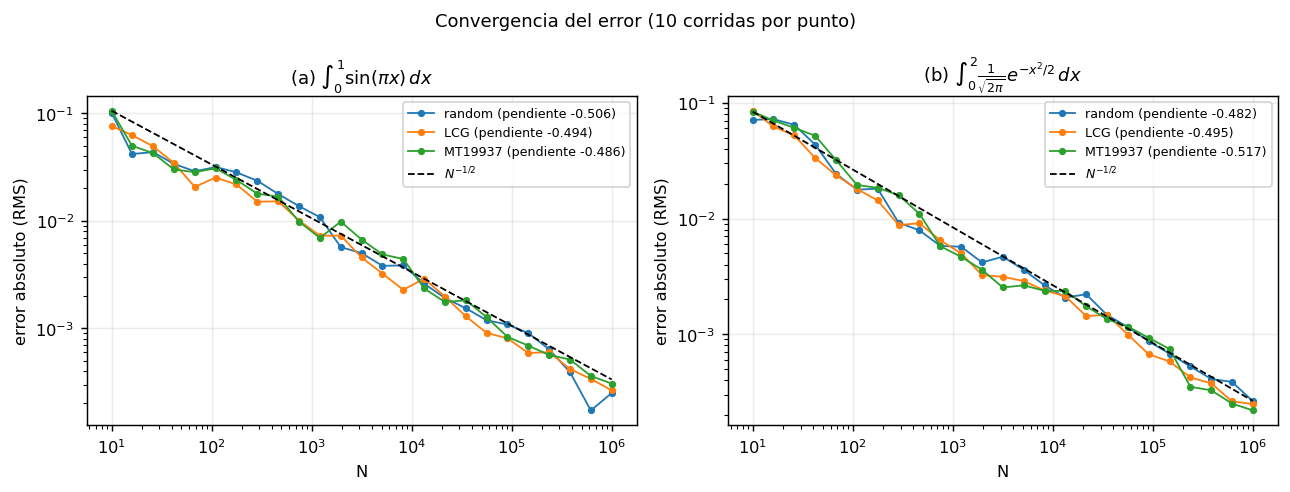
\includegraphics[width=\textwidth]{convergencia_1d.png}
\caption{Error absoluto contra $N$ en escala log--log, promediado sobre
\Repeticiones{} corridas independientes por punto. La recta punteada es la
referencia $N^{-1/2}$.}
\label{fig:convergencia}
\end{figure}

% Generado por los scripts de src/.
% No editar a mano: se sobrescribe en cada ejecucion.
\begin{table}[htbp]\centering
\caption{Pendiente ajustada al error RMS en escala log--log. El valor teorico es $-0.5$.}
\label{tab:pendientes}
\begin{tabular}{l|r|r}
\toprule
Fuente & Integral (a) & Integral (b) \\
\midrule
\texttt{random} & -0.506 & -0.482 \\
\texttt{LCG} & -0.494 & -0.495 \\
\texttt{MT19937} & -0.486 & -0.517 \\
\bottomrule
\end{tabular}
\end{table}


\paragraph{Estudio de convergencia.} La figura~\ref{fig:convergencia} barre
$N$ desde $10$ hasta $10^{6}$. Una sola corrida sale utilísima para nada,
porque el error salta muchísimo de un $N$ al siguiente, así que cada punto de
la gráfica es el error cuadrático medio sobre \Repeticiones{} corridas
independientes con semillas distintas. Con eso, las seis rectas ajustadas dan
pendientes entre $-0.48$ y $-0.52$ contra el $-0.5$ teórico, o sea que la
tasa $\mathcal{O}(N^{-1/2})$ que se derivó arriba se cumple a lo largo de
cinco órdenes de magnitud en $N$, desde $10^1$ hasta $10^6$. Para la integral
(a) con MT19937 la pendiente sale
\PendienteSeno{} y para la (b), \PendienteNormal.

Las diferencias respecto a $-0.5$ son de unas dos centésimas y no hay que
leerles nada raro: con \Repeticiones{} corridas, el propio error RMS trae una
incertidumbre relativa cercana al $20\%$, que es lo que se ve como temblor en
la parte izquierda de la gráfica, donde $N$ es chico. Ninguna de las tres
fuentes da señales de salirse de la tasa teórica.

\paragraph{Comparación entre generadores.} Este resultado hay que subrayarlo
porque a primera vista parece contradecir toda la Parte 1: para estas dos
integrales, el LCG propio funciona igual de bien que \code{random}. ¿Y
entonces para qué tanto escándalo con la calidad de los generadores?

La explicación es que los dos integrandos son funciones suaves de \emph{una}
sola variable, así que el estimador nada más usa la distribución marginal de
cada $u_i$ por separado, y en eso los tres generadores son indistinguibles.
Los defectos de correlación entre valores consecutivos, que es justo donde se
rompen los generadores malos, en este problema ni se activan. Moraleja
provisional: un generador mediocre puede funcionar perfecto mientras el
problema no toque su punto débil. La sección~\ref{sec:randu2} arma a
propósito el caso contrario.

% ---------------------------------------------------------------------------
\subsection{Alta dimensión y la maldición de la dimensionalidad}
\label{sec:altadim}

El volumen de la bola unitaria en $d$ dimensiones es
\begin{equation}
V_d = \int_{[-1,1]^d} \mathbf{1}\big[x_1^2+\dots+x_d^2 \le 1\big]\,d\mathbf{x}
= \frac{\pi^{d/2}}{\Gamma\!\left(\frac{d}{2}+1\right)}.
\label{eq:vol}
\end{equation}
La fórmula cerrada se usa sólo como verdad de referencia. El estimador
muestrea puntos uniformes en el cubo $[-1,1]^d$ y cuenta la fracción
$\hat{p}$ que cae dentro de la bola, de modo que $\hat{V}_d = 2^d \hat{p}$,
con el intervalo de confianza para proporciones de la sección anterior.

% Generado por los scripts de src/.
% No editar a mano: se sobrescribe en cada ejecucion.
\begin{table}[htbp]\centering
\caption{Volumen de la bola unitaria estimado con $N=\NDim$ puntos uniformes en $[-1,1]^d$.}
\label{tab:volumenes}
\small
\begin{tabular}{r|r|r|r|l|l}
\toprule
$d$ & $V_d$ exacto & Aciertos & Estimacion & IC $95\%$ & Error \\
\midrule
2 & 3.1416 & 157{,}047 & 3.1409 & $[3.1337,\ 3.1481]$ & 0.0007 \\
5 & 5.2638 & 32{,}862 & 5.2579 & $[5.2060,\ 5.3099]$ & 0.0059 \\
10 & 2.5502 & 490 & 2.5088 & $[2.2869,\ 2.7307]$ & 0.0414 \\
20 & 0.0258 & 0 & 0.0000 & $[0,\ 15.7286]$ & 0.0258 \\
\bottomrule
\end{tabular}
\end{table}


El deterioro se ve clarísimo y va en dos etapas. Hasta $d=5$ la estimación
sale excelente y uno diría que no hay problema. En $d=10$ el error relativo
ya es de casi $2\%$ a pesar de estar usando $N = \NDim$ puntos, y la razón se
lee en la columna de aciertos: de todos esos puntos, sólo 490 cayeron dentro
de la bola. Y en $d=20$ pasa lo que tenía que pasar: el estimador devuelve
exactamente cero, porque de los \NDim{} puntos, \AciertosVeinte{} cayeron
dentro. Ahí el intervalo normal se degenera, así que hay que reportar la cota
de la regla de tres, $\hat{V}_{20} \le \CotaVeinte$. Técnicamente esa cota sí
contiene al valor verdadero $V_{20} = \ExactoVeinte$, pero es tan ancha que
resulta inútil: es unas $600$ veces más grande que la cantidad que se quería
medir, así que no descarta prácticamente ningún valor.

\begin{figure}[htbp]
\centering
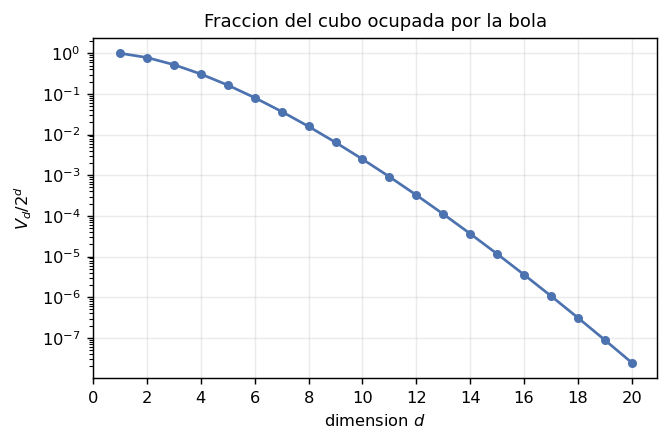
\includegraphics[width=0.62\textwidth]{fraccion_bola.png}
\caption{Fracción del volumen del cubo $[-1,1]^d$ que ocupa la bola unitaria,
en escala logarítmica.}
\label{fig:fraccion}
\end{figure}

\paragraph{Lo que está pasando geométricamente.} La
figura~\ref{fig:fraccion} explica el porqué de todo esto. La razón $V_d/2^d$
se desploma de manera superexponencial: vale $2.49\times 10^{-3}$ en $d=10$ y
\FraccionVeinte{} en $d=20$. En veinte dimensiones la bola inscrita ocupa
una parte en cuarenta millones del cubo que la contiene,
lo cual es bastante difícil de creer viniendo de la intuición de dos o tres
dimensiones, donde la bola se come más de la mitad del cuadrado o del cubo.

¿A dónde se fue todo el volumen? A las esquinas. Hay $2^{20}$ de ellas, y
mientras la distancia del centro a una cara sigue siendo $1$, la distancia a
una esquina es $\sqrt{d}$. Entonces el cubo en dimensión alta no se parece en
nada a un cubo de juguete: es una figura puntiaguda, con casi todo su
contenido lejos del centro.

Para el diseño del estimador esto es letal. El muestreo uniforme en el cubo
está gastando prácticamente todos sus puntos en una región que no aporta nada
al resultado: para pescar \emph{un solo} acierto en $d=20$ harían falta como
\MuestrasUnAcierto{} puntos. El estimador no está roto, está mal escogido
para el problema, y la salida no es subir $N$ como bruto sino cambiar la
distribución de muestreo por una que ponga los puntos donde está la masa, que
es precisamente la idea del muestreo por importancia.

Y un matiz importante para no contradecir lo que se derivó antes: la tasa
sigue siendo $\mathcal{O}(N^{-1/2})$ en cualquier dimensión. Lo que empeora
es la \emph{constante} $\sigma$, porque para un indicador con probabilidad
$p$ chiquita el error relativo es $\sqrt{(1-p)/(pN)}$, que crece como
$1/\sqrt{p}$. La dimensión no ataca al exponente, le pega a la constante.

% Generado por los scripts de src/.
% No editar a mano: se sobrescribe en cada ejecucion.
\begin{table}[htbp]\centering
\caption{Monte Carlo contra cuadratura en rejilla con el mismo presupuesto de puntos, y puntos que exigiria una rejilla de $m=10$ subdivisiones por eje.}
\label{tab:rejilla}
\small
\begin{tabular}{rrrrrr}
\toprule
$d$ & $m$ posible & Puntos usados & Error rejilla & Error MC & Puntos si $m=10$ \\
\midrule
2 & 316 & 99{,}856 & 0.0012 & 0.0007 & $10^{2}$ \\
5 & 10 & 100{,}000 & 0.3793 & 0.0059 & $10^{5}$ \\
10 & 3 & 59{,}049 & 0.9355 & 0.0414 & $10^{10}$ \\
20 & 1 & 1 & 1048575.9742 & 0.0258 & $10^{20}$ \\
\bottomrule
\end{tabular}
\end{table}


\paragraph{Comparación contra la rejilla.} Con el mismo presupuesto de
\Presupuesto{} puntos, la cuadratura determinista evalúa el integrando en el
centro de cada celda de una rejilla de $m$ subdivisiones por eje, con
$m = \lfloor \Presupuesto^{1/d}\rfloor$. En $d=2$ la rejilla gana, como era
de esperarse: con $m = 316$ subdivisiones el error es comparable al de Monte
Carlo. El problema es que ese presupuesto hay que repartirlo entre todos los
ejes, así que $m$ se viene abajo apenas crece $d$: en $d=5$ ya sólo alcanza
para $m=10$, en $d=10$ para $m=3$ y en $d=20$ para $m=1$. Ese último caso es
casi cómico. La rejilla de un solo punto evalúa el integrando en el centro
del cubo, que sí está dentro de la bola, concluye alegremente que
\emph{todo} el cubo está dentro y devuelve
$\hat{V}_{20} = 2^{20} \approx 1.05\times 10^6$ cuando el valor real es
\ExactoVeinte. El resultado es unas $4\times 10^{7}$ veces más grande que el
verdadero y, peor todavía, lo entrega sin ninguna señal de alarma: un método
determinista no trae intervalo de confianza que avise que algo anda mal.

La última columna de la tabla~\ref{tab:rejilla} es el argumento en su versión
más limpia. Para mantener una resolución fija de $m=10$ subdivisiones por eje
hacen falta $10^d$ puntos: son $100$ en dos dimensiones, $10^{10}$ en diez y
$10^{20}$ en veinte, que es más de lo que cualquier computadora va a evaluar
en lo que a uno le queda de vida. Eso es la maldición de la dimensionalidad:
cubrir el espacio con resolución fija cuesta exponencialmente en $d$,
mientras que a Monte Carlo la dimensión sólo lo toca a través de $\sigma$.

\begin{figure}[htbp]
\centering
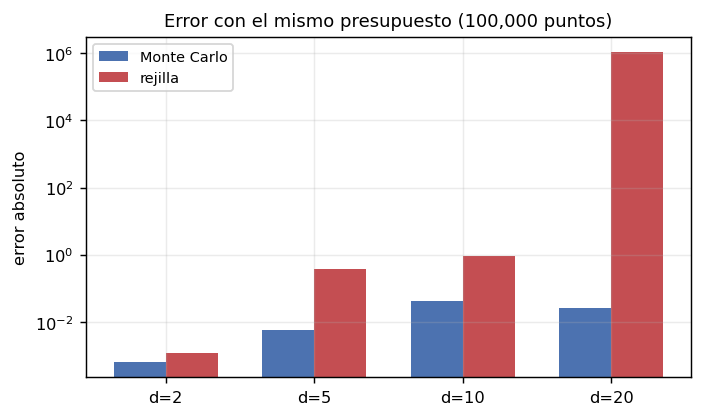
\includegraphics[width=0.66\textwidth]{error_mc_vs_rejilla.png}
\caption{Error absoluto de los dos métodos con el mismo presupuesto de
puntos, en escala logarítmica.}
\label{fig:errorrejilla}
\end{figure}

% ---------------------------------------------------------------------------
\subsection{Reducción de varianza}

Como el error estándar es $(b-a)\sigma/\sqrt{N}$, hay exactamente dos maneras
de reducirlo: subir $N$, que es caro y sólo paga $\sqrt{N}$, o bajar
$\sigma$, que puede pagar mucho más. Se implementaron dos técnicas y se
aplicaron a las dos integrales de la sección anterior, siempre con el mismo
número de evaluaciones de $f$ para que la comparación sea justa.

\subsubsection{Variables antitéticas}

En lugar de promediar $N$ evaluaciones independientes, se generan $N/2$
parejas $(U, 1-U)$, que tienen la misma distribución marginal pero están
negativamente relacionadas, y se promedia dentro de cada pareja:
\begin{equation}
W = \frac{f(U) + f(1-U)}{2},
\qquad \hat{I}^{\,\text{ant}} = \frac{b-a}{N/2}\sum_{j=1}^{N/2} W_j.
\end{equation}
Como $U$ y $1-U$ son ambas uniformes, el estimador sigue siendo insesgado.
Su varianza es
\begin{equation}
\Var(W) = \frac{1}{4}\Big(\Var(f(U)) + \Var(f(1-U)) + 2\Cov(f(U), f(1-U))\Big)
= \frac{\sigma^2(1+\rho)}{2},
\end{equation}
donde $\rho$ es la correlación entre $f(U)$ y $f(1-U)$. Con el mismo
presupuesto de $N$ evaluaciones se usan $N/2$ parejas, así que
\begin{equation}
\Var(\hat{I}^{\,\text{ant}}) = \frac{2}{N}\cdot\frac{\sigma^2(1+\rho)}{2}
= \frac{\sigma^2(1+\rho)}{N},
\qquad
\text{factor de reducción} = \frac{1}{1+\rho}.
\label{eq:antiteticas}
\end{equation}
La conclusión no puede ser más clara: la técnica ayuda si y sólo si
$\rho < 0$, o sea si $f$ es monótona o al menos se comporta al revés en los
dos extremos del intervalo. Si $\rho > 0$, no es que no ayude, es que
empeora. Esto va a importar en un momento.

\subsubsection{Variables de control}

Se busca una función $h$ cuyo valor esperado $\mathbb{E}[h(U)]$ se conozca
exactamente y que esté muy correlacionada con $f$. Se define
\begin{equation}
Y = f(U) - c\,\big(h(U) - \mathbb{E}[h(U)]\big).
\end{equation}
Como el término restado tiene valor esperado cero, $\mathbb{E}[Y] =
\mathbb{E}[f(U)]$ para cualquier constante $c$: el estimador es insesgado sin
importar qué tan buena sea la elección de $h$. Lo que sí depende de $c$ es la
varianza,
\begin{equation}
\Var(Y) = \sigma^2 - 2c\,\Cov(f,h) + c^2\Var(h),
\end{equation}
que es una parábola en $c$ y se minimiza en
\begin{equation}
c^{*} = \frac{\Cov(f,h)}{\Var(h)},
\qquad\text{con}\qquad
\Var(Y)\big|_{c^*} = \sigma^2\big(1-\rho_{f,h}^2\big),
\label{eq:control}
\end{equation}
donde $\rho_{f,h}$ es la correlación entre $f(U)$ y $h(U)$. El factor de
reducción queda entonces en $1/(1-\rho^2)$, que crece sin límite conforme la
correlación se acerca a $\pm 1$. Lo que se gana es toda la parte de $f$ que
$h$ alcanza a explicar: sólo queda por estimar el residuo. El coeficiente
$c^*$ se estimó con una muestra piloto aparte de $20\,000$ puntos, para no
usar los mismos datos dos veces.

Los controles elegidos fueron $h(x) = x(1-x)$ para la integral (a), con
$\mathbb{E}[h] = 1/6$ sobre $\mathrm{Unif}(0,1)$, y $h(x) = x^2$ para la (b),
con $\mathbb{E}[h] = 4/3$ sobre $\mathrm{Unif}(0,2)$. Ambos son polinomios
cuya integral es elemental, que es justamente lo que se necesita: un control
sirve sólo si su valor esperado se conoce de antemano.

\subsubsection{Resultados}

% Generado por los scripts de src/.
% No editar a mano: se sobrescribe en cada ejecucion.
\begin{table}[htbp]\centering
\caption{Reduccion de varianza con $N=\NVar$ evaluaciones de $f$ por estimador, sobre la integral (a) del seno y la (b) de la densidad normal. El factor compara la varianza del estimador contra Monte Carlo simple, y el speedup efectivo es el numero de muestras simples que harian falta para igualar esa precision.}
\label{tab:varianza}
\footnotesize
\begin{tabular}{l|l|r|l|r|r|r}
\toprule
Integral & Tecnica & Estimacion & IC $95\%$ & Varianza & Factor & Speedup \\
\midrule
(a) & simple & $0.636179$ & $[0.634830,\ 0.637528]$ & $4.74\times 10^{-7}$ & 1.00x & $2.0\times 10^{5}$ \\
 & antiteticas & $0.635877$ & $[0.633970,\ 0.637785]$ & $9.47\times 10^{-7}$ & 0.50x & $1.0\times 10^{5}$ \\
 & control & $0.636603$ & $[0.636527,\ 0.636678]$ & $1.49\times 10^{-9}$ & 318.55x & $6.4\times 10^{7}$ \\
\addlinespace
(b) & simple & $0.477290$ & $[0.476280,\ 0.478299]$ & $2.65\times 10^{-7}$ & 1.00x & $2.0\times 10^{5}$ \\
 & antiteticas & $0.477234$ & $[0.477181,\ 0.477287]$ & $7.31\times 10^{-10}$ & 363.07x & $7.3\times 10^{7}$ \\
 & control & $0.477307$ & $[0.477073,\ 0.477542]$ & $1.43\times 10^{-8}$ & 18.54x & $3.7\times 10^{6}$ \\
\addlinespace
\bottomrule
\end{tabular}
\end{table}


\begin{figure}[htbp]
\centering
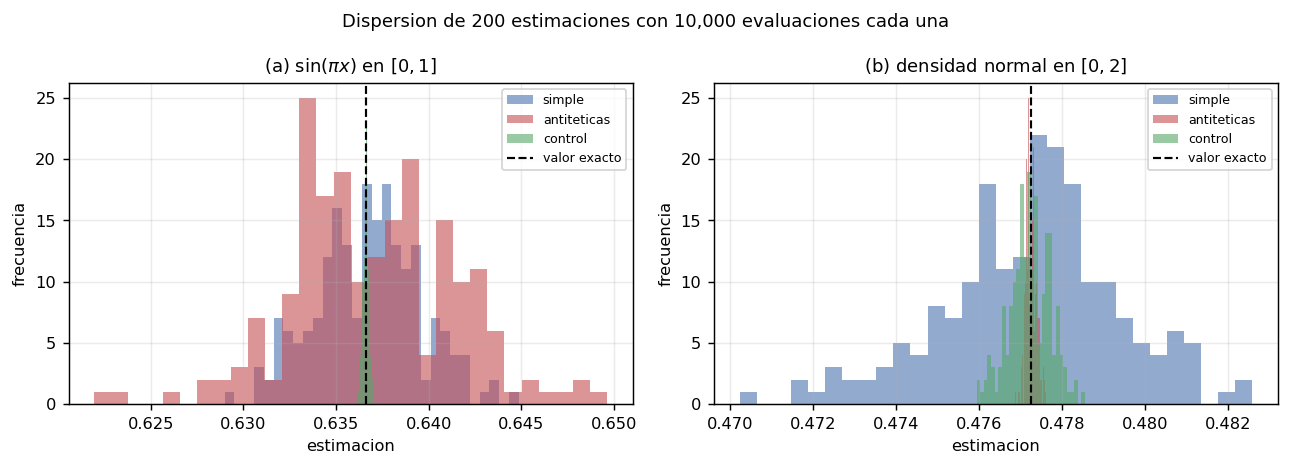
\includegraphics[width=\textwidth]{reduccion_varianza.png}
\caption{Dispersión de \KRepeticiones{} estimaciones independientes con
\NRep{} evaluaciones cada una. Cuanto más angosto el histograma, menor la
varianza del estimador.}
\label{fig:varianza}
\end{figure}

Los cuatro resultados de la tabla~\ref{tab:varianza} le pegan a las fórmulas
\eqref{eq:antiteticas} y \eqref{eq:control} casi al decimal, sin haber
acomodado nada:

\begin{itemize}[itemsep=3pt]
  \item \textbf{Antitéticas en la integral (b): \FactorAntiNormal x.} La
        densidad normal es estrictamente decreciente en $[0,2]$, así que
        $f(U)$ y $f(2-U)$ están fuertemente correlacionadas de forma
        negativa. La reducción es de más de dos órdenes de magnitud y sale
        gratis: no requiere información adicional sobre el integrando, sólo
        saber que es monótono.
  \item \textbf{Antitéticas en la integral (a): \FactorAntiSeno x, es decir,
        empeora.} Aquí está la respuesta a la pregunta de si la técnica
        siempre ayuda. La función $\sin(\pi x)$ es simétrica respecto a
        $x = 1/2$, de modo que $f(1-U) = f(U)$ \emph{exactamente} y por lo
        tanto $\rho = +1$. La fórmula~\eqref{eq:antiteticas} predice un
        factor de $1/(1+1) = 0.5$, y lo medido es \FactorAntiSeno x. El
        estimador gasta dos evaluaciones para obtener la información de una:
        la pareja antitética es una copia idéntica.
  \item \textbf{Control en la integral (a): \FactorControlSeno x.} La
        correlación medida entre $\sin(\pi x)$ y $x(1-x)$ es
        $\rho = \CorrSeno$, porque ambas son campanas simétricas que se
        anulan en los extremos. La fórmula predice
        $1/(1-\CorrSeno^2) \approx 313$ y lo medido es
        \FactorControlSeno x.
  \item \textbf{Control en la integral (b): \FactorControlNormal x.} La
        correlación con $x^2$ es $\CorrNormal$ y la predicción
        $1/(1-\rho^2) \approx 18.8$ coincide con lo medido.
\end{itemize}

\paragraph{Qué significa eso en muestras.} Un factor de reducción $F$ quiere
decir que la técnica llega, con $N$ evaluaciones, a la misma precisión que
Monte Carlo simple alcanzaría con $F\cdot N$. Ése es el speedup efectivo y
aparece en la última columna de la tabla~\ref{tab:varianza}, expresado
directamente en muestras simples equivalentes. Para el control en la integral
(a), igualar por fuerza bruta la precisión que se obtuvo con $N = \NVar$
muestras pediría alrededor de $6\times10^{7}$ muestras simples. Ahí está el
argumento económico de toda la sección: media hora pensando en un buen
control vale más que dejar la computadora corriendo toda la noche.

\paragraph{¿Entonces siempre conviene usarlas?} No, y cada técnica falla por
un motivo distinto. Las antitéticas dependen del \emph{signo} de $\rho$:
ayudan con integrandos monótonos y estorban con integrandos simétricos, que
es exactamente lo que se vio arriba. Las variables de control dependen de la
\emph{magnitud} de $\rho$ y además piden conocer $\mathbb{E}[h]$ de antemano;
si uno elige un control con correlación cercana a cero, el factor
$1/(1-\rho^2)$ se va a $1$ y no se gana nada, aunque al menos tampoco se
pierde el insesgamiento. En los dos casos lo que manda es la forma del
integrando, no la técnica, así que el orden correcto de trabajo es mirar
primero cómo es $f$ y después decidir.

% ---------------------------------------------------------------------------
\subsection{Cuando el generador arruina el resultado: el caso RANDU}
\label{sec:randu2}

En la Parte 1 quedó demostrado que las ternas consecutivas de RANDU caen en
\PlanosRandu{} planos del cubo $[0,1]^3$, y también que las cuatro pruebas de
hipótesis no detectan nada. Falta ver qué le hace eso a un cálculo real. Se
estimaron dos volúmenes en tres dimensiones, ambos con ternas consecutivas
$(u_i, u_{i+1}, u_{i+2})$ y $N = \NRandu$ ternas por estimación:
\begin{align}
\text{(i) } &\int_{[0,1]^3}\mathbf{1}\big[x^2+y^2+z^2 \le 1\big]\,dx\,dy\,dz
= \frac{\pi}{6} = \ExactoOctante, \\
\text{(ii) } &\int_{[0,1]^3}\mathbf{1}\big[x^2+y^2+z^2 \le r^2\big]
\,dx\,dy\,dz = \frac{\pi r^3}{6} = \ExactoBola,
\qquad r = \RadioBola.
\end{align}
El primero es el octante de la bola unitaria; el segundo es una bola pequeña
pegada al origen. Los dos se estimaron con RANDU y con el Mersenne Twister.

% Generado por los scripts de src/.
% No editar a mano: se sobrescribe en cada ejecucion.
\begin{table}[htbp]\centering
\caption{Dos estimaciones en tres dimensiones con $N=\NRandu$ ternas consecutivas de cada generador. La ultima columna es la fraccion de los $K=\KRandu$ intervalos que cubren el valor real.}
\label{tab:randu}
\small
\begin{tabular}{l|l|r|l|r|r|c}
\toprule
Region & Fuente & Estimacion & IC $95\%$ & Sesgo relativo & $|z|$ & Cobertura \\
\midrule
Bola unitaria & RANDU & $0.523444$ & $[0.522752,\ 0.524137]$ & $-0.03\%$ & $0.4$ & 96\% \\
Bola unitaria & Mersenne Twister & $0.524037$ & $[0.523345,\ 0.524729]$ & $+0.08\%$ & $1.2$ & 97\% \\
\addlinespace
Bola $r=0.1$ & RANDU & $0.000654$ & $[0.000619,\ 0.000689]$ & $+24.90\%$ & $7.2$ & 87\% \\
Bola $r=0.1$ & Mersenne Twister & $0.000532$ & $[0.000500,\ 0.000564]$ & $+1.60\%$ & $0.5$ & 93\% \\
\addlinespace
\bottomrule
\end{tabular}
\end{table}


\begin{figure}[htbp]
\centering
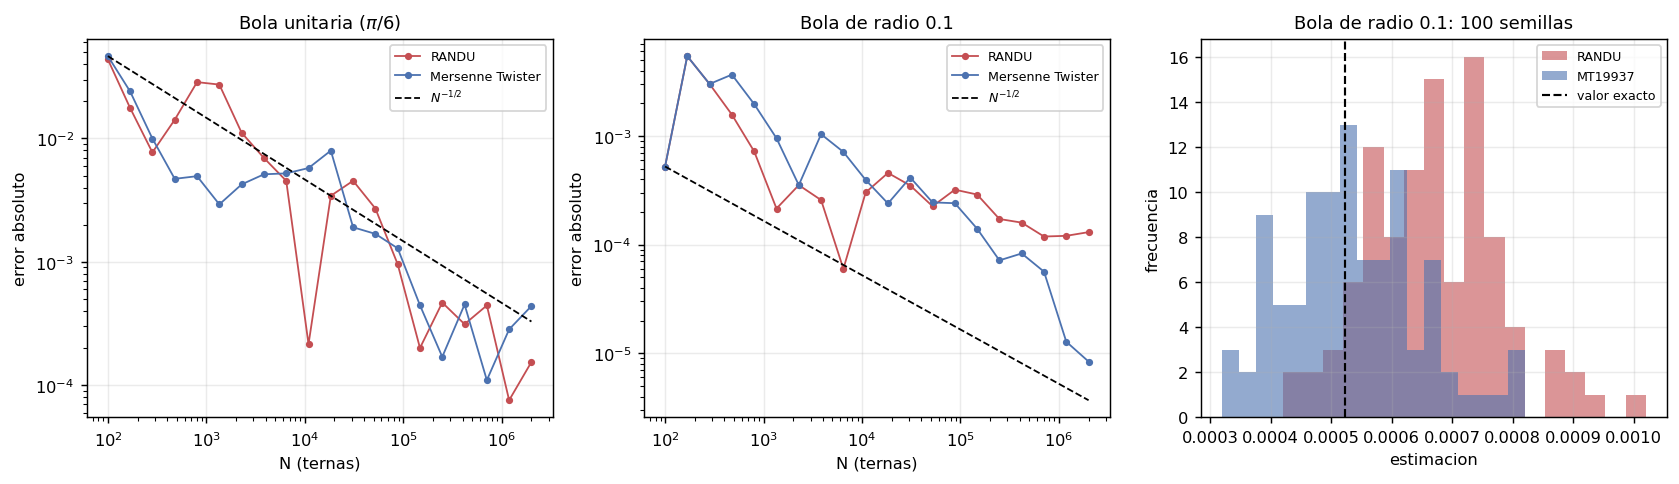
\includegraphics[width=\textwidth]{randu_montecarlo.png}
\caption{Izquierda y centro: error absoluto contra el número de ternas, en
escala log--log. Derecha: dispersión de las estimaciones de la bola pequeña
sobre \KRandu{} semillas distintas.}
\label{fig:randumc}
\end{figure}

\paragraph{Lo que pasó con la región grande.} Con el octante de la bola
unitaria, RANDU y el Mersenne Twister dan prácticamente lo mismo:
$\EstRanduOctante$ contra $\EstMTOctante$, los dos a menos de dos errores
estándar del valor exacto y los dos con intervalos que lo cubren. En el panel
izquierdo de la figura~\ref{fig:randumc} las dos curvas de error bajan
pegaditas a la referencia $N^{-1/2}$. Si el análisis se hubiera quedado aquí,
la conclusión habría sido que RANDU funciona sin problema, que es justo lo
que le pasó a mucha gente en los años 60.

\paragraph{Lo que pasó con la región pequeña.} Con la bola de radio
$r = \RadioBola$ la historia cambia por completo. RANDU estima
$\EstRanduBola$ cuando el valor real es $\ExactoBola$: un sesgo relativo de
\RelativoRanduBola, o sea que se equivoca por una cuarta parte del valor. Su
intervalo de confianza, $\ICRanduBola$, \textbf{no contiene} el valor
verdadero, y la desviación es de \SigmasRanduBola{} errores estándar, así que
esto no le pasó por mala suerte. Con
exactamente la misma cantidad de ternas, el Mersenne Twister estima
$\EstMTBola$, con un sesgo de \RelativoMTBola{} y una desviación de
\SigmasMTBola{} errores estándar, que es indistinguible de cero. Mismo
código, mismo estimador, misma $N$: lo único que cambió fue quién genera los
números.

El panel central de la figura~\ref{fig:randumc} muestra el síntoma que
delata todo: la curva de RANDU baja al principio y después \textbf{se
aplana}, mientras que la del Mersenne Twister sigue la referencia
$N^{-1/2}$ hasta el final. Y eso es un diagnóstico bastante claro, porque un
error que deja de bajar cuando uno agrega muestras ya no es ruido, es sesgo.
La diferencia importa: el ruido se arregla con más muestras y el sesgo no.
RANDU no está convergiendo despacio hacia el valor correcto, está
convergiendo muy bien hacia un valor equivocado.

\paragraph{Por qué pasa esto, geométricamente.} La respuesta es la
figura~\ref{fig:planos} de la Parte 1, ni más ni menos. Las ternas de RANDU
no viven en el cubo, viven en \PlanosRandu{} planos paralelos de normal
$(9,-6,1)$. Entonces el estimador de Monte Carlo no está midiendo el volumen
de la región: está midiendo qué fracción de \emph{esos planos} cae dentro de
la región, que es otra cosa.

Cuando la región es grande, como el octante de la bola, la cruzan varios
planos y los errores de unos y otros se compensan al promediar, así que el
resultado sale bien casi de milagro. Cuando la región es chica comparada con
la separación entre planos, como la bola de radio $\RadioBola$, apenas unos
pocos planos la atraviesan y la estimación queda a merced de dónde
exactamente caen esos planos. Si pasan cerca del centro, sobra volumen
aparente, y por eso el resultado sale \RelativoRanduBola{} arriba. La
convergencia es real, pero converge a la medida de la intersección de los
planos con la bola, que no es el número que se quería calcular.

\paragraph{Y los intervalos de confianza también se descomponen.} La última
columna de la tabla~\ref{tab:randu} repite cada estimación con \KRandu{}
semillas distintas y cuenta cuántos de esos intervalos del $95\%$ contienen
al valor real. Con el octante los dos generadores se portan bien
(\CoberturaRanduOctante{} y \CoberturaMTOctante, que es justo lo que uno
esperaría). Con la bola pequeña, el Mersenne Twister se mantiene en
\CoberturaMTBola{} y RANDU se cae a \CoberturaRanduBola. Esto es lo más grave
de todo el experimento: con RANDU los intervalos dejan de
significar lo que dicen significar. Están reportando una precisión que el
estimador no tiene, y quien lea el resultado no tiene forma de enterarse.

\paragraph{Cómo se conecta todo esto con la Parte 1.} Con esto se cierra el
círculo que quedó abierto en la sección~\ref{sec:randu}. Las cuatro pruebas
de hipótesis miraban un valor o una pareja a la vez, y por eso le dieron el
visto bueno a RANDU. La prueba espectral, que sí mira ternas, lo reprobó de
inmediato. Y el cálculo de Monte Carlo de esta sección es un problema
genuinamente tridimensional, así que era de esperarse que repitiera el
veredicto de la prueba espectral y no el de las pruebas de hipótesis. La
correspondencia no es casualidad, y de ahí sale una regla práctica bastante
útil: la herramienta con la que uno diagnostica un generador tiene que mirar
la misma dimensión en la que lo va a usar.

% ===========================================================================
\newpage
\section{Conclusiones}

De todo lo anterior salen cuatro conclusiones.

\textbf{Uniformidad e independencia son cosas distintas, y la difícil es la
segunda.} Los cinco generadores se dividen en tres grupos según cómo fallan.
Cuadrados medios falla de la forma más burda que existe: se muere. LCG,
Mersenne Twister y Blum Blum Shub pasan las cuatro pruebas, cada uno con su
propio trato entre velocidad, período y seguridad. Y RANDU también las pasa,
con $p$-valores de lo más respetables, mientras esconde una identidad
algebraica que lo tiene encerrado en \PlanosRandu{} planos. Entonces una
batería de pruebas se lee distinto de como uno esperaría: que un generador
pase cuatro pruebas unidimensionales no es evidencia de que sea bueno, sino
de que no se le encontró el defecto con las herramientas que se usaron, que
no es lo mismo.

\textbf{La teoría es la que dice dónde mirar.} El defecto de RANDU no
apareció explorando datos, apareció haciendo el álgebra de
$a^2 \equiv 6a - 9$. Con Blum Blum Shub pasó igual: la diferencia entre un
generador que funciona y uno que cicla en treinta estados no estaba en el
código sino en cómo se factoriza $\lambda(\lambda(N))$, y eso no se descubre
graficando. Y el período de $2^{19937}-1$ del Mersenne Twister no es algo que
alguien haya medido, es una afirmación sobre la primitividad de un polinomio.
En los tres casos, primero está la matemática y después el experimento.

\textbf{Monte Carlo es lento, pero le da igual la dimensión.} La tasa
$\mathcal{O}(N^{-1/2})$ que derivamos y verificamos es mala comparada con
cualquier cuadratura en una dimensión, y aun así no depende de $d$. Cuando
uno ve que la rejilla necesita $10^{20}$ puntos para tener diez subdivisiones
por eje en veinte dimensiones, esa indiferencia deja de ser un detalle
técnico y se vuelve la única razón por la que el cálculo se puede hacer. Eso
sí, la dimensión igual cobra lo suyo a través de $\sigma$, y ahí entran las
técnicas de reducción de varianza: bajar la constante salió hasta
\FactorControlSeno{} veces más rentable que subir $N$, pero sólo cuando la
técnica le queda al integrando. Las antitéticas aplicadas a una función
simétrica no ayudaron nada, al contrario, costaron el doble.

\textbf{Un método de Monte Carlo nunca va a ser mejor que su fuente de
aleatoriedad.} El experimento reproduce esta moraleja de forma bastante
limpia. Con una región grande, RANDU da un resultado correcto y
tranquilizador. Con una región chica, el mismo generador, el mismo estimador
y el mismo número de muestras dan un error de \RelativoRanduBola{} que no
baja aunque uno agregue muestras, y un intervalo de confianza que miente. Y
lo más preocupante no es que RANDU falle, porque eso se sabe desde 1968, sino
que falle \emph{en silencio}: sin la fórmula cerrada para comparar, nada en
la salida del programa habría dicho que ese número estaba mal.

% ===========================================================================
\newpage
\section*{Referencias}
\addcontentsline{toc}{section}{Referencias}
\begin{thebibliography}{9}

\bibitem{marsaglia1968}
G. Marsaglia, ``Random Numbers Fall Mainly in the Planes'',
\emph{Proceedings of the National Academy of Sciences}, vol. 61, no. 1,
pp. 25--28, 1968. doi: 10.1073/pnas.61.1.25.

\bibitem{randomorg}
RANDOM.ORG, \emph{Introduction to Randomness and Random Numbers}.
\url{https://www.random.org/randomness/}

\bibitem{matsumoto1998}
M. Matsumoto y T. Nishimura, ``Mersenne Twister: A 623-Dimensionally
Equidistributed Uniform Pseudo-Random Number Generator'',
\emph{ACM Transactions on Modeling and Computer Simulation}, vol. 8, no. 1,
pp. 3--30, 1998.

\bibitem{blum1986}
L. Blum, M. Blum y M. Shub, ``A Simple Unpredictable Pseudo-Random Number
Generator'', \emph{SIAM Journal on Computing}, vol. 15, no. 2, pp. 364--383,
1986.

\bibitem{hulldobell}
T. E. Hull y A. R. Dobell, ``Random Number Generators'',
\emph{SIAM Review}, vol. 4, no. 3, pp. 230--254, 1962.

\bibitem{knuth}
D. E. Knuth, \emph{The Art of Computer Programming, Volume 2:
Seminumerical Algorithms}, 3a ed., Addison-Wesley, 1997.

\bibitem{press2007}
W. H. Press, S. A. Teukolsky, W. T. Vetterling y B. P. Flannery,
\emph{Numerical Recipes: The Art of Scientific Computing}, 3a ed.,
Cambridge University Press, 2007.

\bibitem{owen2013}
A. B. Owen, \emph{Monte Carlo Theory, Methods and Examples}, 2013.

\end{thebibliography}

\end{document}
